%%%%%%%%%%%%%%%%%%%%%%%%%%%%%%%%%%%%%%%%%%%%%%%%%%%%%%%%%%%%%%%%%%%
%                                                                 %
%   HBOOK User Guide -- LaTeX Source                              %
%                                                                 %
%   Chapter 7                                                     %
%                                                                 %
%   The following external EPS files are referenced:              %
%           fhtest4.eps, fhtest5.eps, fhtest6.eps                 %
%                                                                 %
%   Editor: Michel Goossens / CN-AS                               %
%   Last Mod.: 14 Jan 1997  11:45 mg                               %
%                                                                 %
%%%%%%%%%%%%%%%%%%%%%%%%%%%%%%%%%%%%%%%%%%%%%%%%%%%%%%%%%%%%%%%%%%%
 
\Filename{H1Fitting-parameterization-and-smoothing}
\chapter{Fitting, parameterization and smoothing}
\label{HFITPASM}

\Filename{H2Fitting}
\section{Fitting}
\label{HFitting}
\index{fitting|(}
 
The fitting routines in HBOOK are based 
on the Minuit package \cite{bib-MINUIT}.
Minuit is conceived as a tool to find the minimum
value of a
\index{minimisation}
\index{fit}
multi-parameter function and analyze the shape of the function
around the minimum. The principal application is foreseen for
statistical analysis, working on chisquare or
log-likelihood functions,
to compute the best-fit parameter values and uncertainties,
including correlations between the parameters.
It is especially suited to handle difficult problems, including those
which may require guidance in order to find the correct solution.

In the case of \(\chi^2\) minimization, 
the final fitted parameter values correspond to
the minimum of the \(\chi^2\) function as defined below:
 
\begin{displaymath}
\chi^{2}\, =\, \sum_{i=1}^{n}
                \left(\,
                   \frac{\displaystyle\mathtt{C(I)}
                         -F(\mathrm{X(I)},A_1,A_2,...,A_k)}
                        {\displaystyle\mathtt{E(I)}}
                \right)^{2}
\end{displaymath}
 
where the following definitions are used:
 
\begin{DLtt}{1234567}
\item[n]    Number of channels (cells) in the 1-dimensional or 2-dimensional
            histogram (\Rind{HFITH}, \Rind{HFITHN}) or
            number of points of the distribution (\Rind{HFITV})
\item[C(I)] Contents of channel (cell) \Lit{I}
\item[E(I)] Error on \Lit{C(I)}
\item[X(I)] Coordinate(s) of centre of channel (cell) \Lit{I} or
            coordinate vector of point \Lit{I} of the distribution
\item[$A_1..A_k$] Parameters of the parametric function.
\item[$F$]  Parametric function to be fitted to the data points.
\end{DLtt}
 
\Remarks
\begin{UL}
\item If no errors are specified by the user,
      they are taken to be the square root of the bin contents.
      In this case:
      \begin{UL}
      \item empty channels are ignored by the fitting procedure;
      \item If at least one of \Lit{C(I)<0}, then \Lit{E(I)} is
            set to 1 for all channels (cells).
      \end{UL}
\item If errors are correctly defined via \Rind{HBARX} or \Rind{HPAKE},
      then all channels will be taken into account.
\end{UL}
 
The minimization algorithm requires the calculation of derivatives of
the function with respect to the parameters and this is normally done
numerically by the fitting routine. If the analytical expression of the
derivatives is known, the fit can be speeded up by making use of this
information (see option \Lit{D} in the control flag of the
various fitting routines).
 
For a log-likelihood fit, the likelihood 
is formed by determining the Poisson
probability that given a number of entries in a particualar bin,
the fit would predict its value.  This is then done for each bin,
and the sum of the logs is taken as the likelihood.
\index{log-likelihood}
\index{Poisson distribution}

\newpage
\subsection{One and two-dimensional distributions}

\Shubr{HFITH}{(ID,FUN,CHOPT,NP,*PARAM*,STEP,PMIN,PMAX,SIGPAR*,CHI2*)}
 
\Action
Fits a given parametric function to the contents of a
1- or 2-dimensional histogram, and optionally superimposes
it to the 1-dimensional histogram when editing.
 
\begin{DLtt}{12345}
\item[{\rm\bf Input parameters:}]
\item[ID] Histogram identifier.
\item[FUN] Parametric function (to be declared \Lit{EXTERNAL},
           see \ref{sec:userparfun})           \\
           Can be defined interactively in the interactive version 
           (see \PAW{} manual)
\item[CHOPT] Character variable specifying the desired options.
\begin{DLtt}{1234}
\item['B'] Some or all parameters are bounded.
           The arrays \Lit{STEP}, \Lit{PMIN} and \Lit{PMAX}
           must be specified.
           By default all parameters vary freely.
\item['D'] The user specifies the derivatives of the function
           analytically by providing the user routine \Rind{HDERIV}.
           By default derivatives are computed numerically.
\item['E'] Perform a detailed error analysis using the MINUIT routines
           \Rind{HESSE} and \Rind{MINOS}
\item['F'] Force storing of the result of the fit bin by bin with the
           histogram for an any-dimensional histogram.
\item['K'] \Lit{'KM'} means: do to reset the parameters of 
           \Lit{Application HMINUIT}.
\item['L'] Use the logaritmic Likelihood fitting method.
           By default the chisquared method is used.
\item['M'] Invoke interactive \Lit{MINUIT}.
\item['N'] The results of the fit are not stored
           bin by bin with the histogram.
           By default the function is calculated at the centre of each bin
           in the specified range.
\item['Q'] Quiet mode. No printing.
\item['R'] Fit a Restricted area of a 1-D or 2-D histogram.
           The limits for the fit are given using in the vector \Lit{IQUEST} 
           is in the communication common \Lit{/QUEST/IQUEST(100)}, as follows:\\
\index{IQUEST@{\tt IQUEST} communication vector}%
           \Lit{IFXLOW = IQUEST(11)} specifies the lower limit in X,\\
           \Lit{IFXUP  = IQUEST(12)} specifies the upper limit in X,\\
           \Lit{IFYLOW = IQUEST(13)} specifies the lower limit in Y (2-D),\\
           \Lit{IFYUP  = IQUEST(14)} specifies the upper limit in Y (2-D).
\item['U'] User function value is taken from \Lit{/HCFITD/FITPAD(24),FITFUN},
\index{HCFITD@{\tt /HCFITD/} fit parameters common}%
           see section~\ref{sec:userparfun}.
           All calculations are performed in double precision.
\item['V'] Verbose mode.
           Results are printed after each iteration.
           By default only final results are printed.
\item['W'] Set the event weights equal to one.
           By default weights are taken according to statistical errors.
%\item['T'] Routine \Lit{HFITH} is invoked from another HBOOK routine.
%           In this case parameter names are taken from \Lit{/HCFITS/}.
\end{DLtt}
\item[NP]  Number of parameters (\Lit{NP\(\leq\)25}).
\item[PARAM] Array of dimension \Lit{NP} with initial values for
      the parameters.
\item[STEP] Array of dimension \Lit{NP} with initial step sizes
      for the parameters (\Lit{'B'} option only).
\item[PMIN] Array of dimension \Lit{NP} with the lower bounds
      for the parameters (\Lit{'B'} option only).
\item[PMAX] Array of dimension \Lit{NP} with the upper bounds
      for the parameters (\Lit{'B'} option only).
\item[{\rm\bf Output parameters:}]
\item[PARAM] Array of dimension \Lit{NP} with the final fitted values
      of the parameters.
\item[SIGPAR] Array of dimension \Lit{NP} with the standard deviations
      on the final fitted values of the parameters.
\item[CHI2] Chisquared of the fit.
\end{DLtt}
 
%\finalnewpage%%%%%%%%%%%%%%%%%%%%%%%%%%%%%%%%%%%%%%%%%%%%%%%%%%%%%%%%%%%

\subsection{Fitting one-dimensional histograms with special functions}

\Shubr{HFITHN}{(ID,CHFUN,CHOPT,NP,*PAR*,STEP,PMIN,PMAX,SIGPAR*,CHI2*)}

\Action
Fits the given special function to the contents of a
one-dimensional histogram, and optionally superimposes
it to the histogram when editing.
 
\begin{DLtt}{12345}
\item[{\rm\bf Input parameters:}]
\item[ID] Histogram identifier.
\item[CHFUN] Character variable specifying the desired parametric function.
      Possible keywords are:
      \begin{DLtt}{123}
      \item[G] to fit gaussian \Lit{PAR(1)*exp(-0.5*((x-PAR(2))/PAR(3))**2)}.\\
      \Lit{PAR(1)} corresponds to the normalization,\\
      \Lit{PAR(2)} corresponds to the mean value, and\\
      \Lit{PAR(3)} corresponds to the half width of the Gaussian.
\index{gaussian!fit}
\index{fit!gaussian}
      \item[E] to fit exponential \Lit{exp(PAR(1)+PAR(2)*x)}
\index{exponential!fit}
\index{fit!exponential}
      \item[Pn] to fit polynomyal \Lit{PAR(1)+PAR(2)*x+PAR(3)*x**2......+PAR(n+1)*x**n}
\index{polynomial!fit}
\index{fit!polynomial}
      \end{DLtt}
      Any combination of these keywords with the 2 operators \Lit{+} or \Lit{*}
      is allowed, e.g. \Lit{'p4+g'}, a combination of a 4th degree polynomial
      and a gaussian, which needs eight parameters or
      \Lit{p2*g+g}, a second degree polynomyal and 2 gaussians,
      needing 9 parameters.
      The order of the parameters in \Lit{PAR} must
      correspond to the order of the basic functions.
      For example, in the first case above, \Lit{PAR(1:5)} apply to
      the polynomial of degree 4 and \Lit{PAR(6:8)} to the gaussian while
      in the second case \Lit{PAR(1:3)} apply to the polynomial of degree 2,
      \Lit{PAR(4:6)} to the first gaussian and \Lit{PAR(7:9)} to the second gaussian.
      Blanks are not allowed in the expression.
\item[CHOPT] 
\begin{DLtt}{1234}
\item['B'] Some or all parameters are bounded.
           The arrays \Lit{STEP}, \Lit{PMIN} and \Lit{PMAX}
           must be specified.
           By default all parameters vary freely.
\item['D'] The user is assumed to compute derivatives analytically
           using the routine \Rind{HDERIV}.
           By default, derivatives are computed numerically.
\item['E'] Perform a detailed error analysis using the \MINUIT{} routines
           \Rind{HESSE} and \Rind{MINOS}
\item['F'] Force storing of the result of the fit bin by bin with the
           histogram.
\item['L'] Use the logaritmic Likelihood fitting method.
           By default the chisquared method is used.
\item['M'] Invoke interactive \MINUIT.
\item['N'] The results of the fit are not stored
           bin by bin with the histogram.
           By default the function is calculated at the centre of each bin
           in the specified range.
\item['Q'] Quiet mode. No printing.
\item['R'] Fit a Restricted area of the 1-D histogram.
           \Lit{IFTLOW = IQUEST(11)} specifies the lower limit of the minimization domain,\\
           \Lit{IFTUP  = IQUEST(12)} specifies the upper limit of the minimization domain.
           \index{IQUEST@{\tt IQUEST} communication vector}
\item['V'] Verbose mode.
           Results are printed after each iteration.
           By default only final results are printed.
\item['W'] Set event weights to one.
           By default weights are taken according to statistical errors.
\end{DLtt}
\item[NP] Number of parameters.
\item[PAR] Array of dimension \Lit{NP} with initial values for
      the parameters.
\item[STEP] Array of dimension \Lit{NP} with initial step sizes
      for the parameters (\Lit{'B'} option only).
\item[PMIN] Array of dimension \Lit{NP} with the lower bounds
      for the parameters (\Lit{'B'} option only).
\item[PMAX] Array of dimension \Lit{NP} with the upper bounds
      for the parameters (\Lit{'B'} option only).

\item[{\rm\bf Output parameters:}]
\item[PAR] Array of dimension \Lit{NP} with the final fitted values
      of the parameters.
\item[SIGPAR] Array of dimension \Lit{NP} with the standard deviations
      on the final fitted values of the parameters.
\item[CHI2] Chisquared of the fit.
\end{DLtt}
 
\subsection{Fitting one or multi-demensional arrays}

\Shubr{HFITV}{(N,NDIM,NVAR,X,Y,EY,FUN,CHOPT,NP,*PAR*,STEP,PMIN,PMAX,SIGPAR*, CHI2*)}
 
\Action
Fits a given parametric function to a number of value pairs
with associated errors.
 
\begin{DLtt}{12345}
\item[{\rm\bf Input parameters:}]
\item[N] Number of points to be fitted.
\item[NDIM] Declared first dimension of array \Lit{X}.
\item[NVAR] Dimension of the distribution.
\item[X] Array of dimension \Lit{N} containing the X-coordinates
      of the points to be fitted.
\item[Y] Array of dimension \Lit{N} containing the Y-coordinates
      of the points to be fitted.
\item[EY] Array of dimension \Lit{N} containing the errors on the
      Y-coordinates of the points to be fitted.
\item[FUN] Parametric function (to be declared \Lit{EXTERNAL})
\item[CHOPT] Character variable specifying the desired options.
\begin{DLtt}{1234}
\item['B'] Some or all parameters are bounded.
           The arrays \Lit{STEP}, \Lit{PMIN} and \Lit{PMAX}
           must be specified.
           By default all parameters vary freely.
\item['D'] The user provides the derivatives of the function
           analytically by specifying the user routine \Rind{HDERIV}.
           By default derivatives are computed numerically.
\item['E'] Perform a detailed error analysis using the \MINUIT{} routines
\item['L'] Use the logaritnic Likelihood fitting method.
           By default the chisquared method is used.
\item['M'] Invoke interactive \Lit{MINUIT}.
\item['Q'] Quiet mode. No printing.
\item['U'] User function value is taken from \Lit{/HCFITD/FITPAD(24),FITFUN},
\index{HCFITD@{\tt /HCFITD/} fit parameters common}%
           see section~\ref{sec:userparfun}.
           All calculations are performed in double precision.
\item['V'] Verbose mode.
           Results are printed after each iteration.
           By default only final results are printed.
\item['W'] Set the event weights equal to one.
           By default weights are taken according to statistical errors.
\Rind{HESSE} and \Rind{MINOS}
\end{DLtt}
\item[NP] Number of parameters (\Lit{NP\(\leq\)25}).
\item[PAR] Array of dimension \Lit{NP} with initial values for
      the parameters.
\item[STEP] Array of dimension \Lit{NP} with initial step sizes
      for the parameters (\Lit{'B'} option only).
\item[PMIN] Array of dimension \Lit{NP} with the lower bounds
      for the parameters (\Lit{'B'} option only).
\item[PMAX] Array of dimension \Lit{NP} with the upper bounds
      for the parameters (\Lit{'B'} option only).
\item[{\rm\bf Output parameters:}]
\item[PAR] Array of dimension \Lit{NP} with the final fitted values
      of the parameters.
\item[SIGPAR] Array of dimension \Lit{NP} with the standard deviations
      on the final fitted values of the parameters.
\item[CHI2] Chisquared of the fit.
\end{DLtt}
 
%\finalnewpage%%%%%%%%%%%%%%%%%%%%%%%%%%%%%%%%%%%%%%%%%%%%%%%%%%%%%%%%%%%


\subsection{Results of the fit}
\label{sec:resultfit}

When the fit is complete, the parameters and the errors on the
parameters are returned to the calling program.
By default (unless option \Ropt{N} is specified),
the fitted parameters, the errors on these parameters,
their names (see below),
the chi-squared and the number of degrees of freedom of the fit
are stored in a data structure associated to the histogram \Lit{ID}
when routines \Rind{HFITH} and \Rind{HFITHN} are invoked.

\begin{UL}
\item For \Rind{HFITH} the value of the fitted function
      in each histogram channel is also stored in the histogram
      data structure.
      The parameters are given the default names:
      \Lit{P1}, \Lit{P2},...,\Lit{Pn}.
\item For \Rind{HFITHN} the type of the function being fitted
      is stored instead of the fitted values for each channel.
\end{UL}

The information stored in the associated data structure is used 
during the printing/plotting phase.
In particular it is written when the histogram is stored in a file
with \Rind{HROUT}.

\subsubsection*{Naming the parameters of a fit}

\Shubr{HFINAM}{(ID,CHPNAM,NPAR)}
 
\Action
Modify the names of the fitted parameters
in the data structure associated with the given histogram.

\begin{DLtt}{123456}
\item[{\rm\bf Input parameter:}]
\item[ID]     Histogram identifier.
\item[CHPNAM] \Lit{CHARACTER} array specifying the name(s) to be given to
              the parameter(s) of the fit (truncated to 8 characters).
\item[NPAR]   Number of parameters specified.
\end{DLtt}

\subsection*{Retrieving the fitted parameters}

\Shubr{HGFIT}{(ID,NFPAR*,NPFITS*,FITCHI*,FITPAR*,FITSIG*,FITNAM*)}

\Action
Retrieve the fitted parameters values
from the data structure associated with a given histogram.

\begin{DLtt}{12345}
\item[\textrm{\textbf{Input parameter:}}]
\item[ID]     Histogram identifier.
\item[\textrm{\textbf{Output parameters:}}]
\item[NFPAR]  Number of parameters.
\item[NPFITS] Number of data points used in the fit.
\item[FITCHI] \(\chi^2\) of the fit.
\item[FITPAR] Array of dimension at least \Rarg{NFPAR},
              containing the value of the fitted parameters.
\item[FITSIG] Array of dimension at least \Rarg{NFPAR},
              containing the standard deviations of
              values of the fitted parameters.
\item[FITNAM] Character array of dimension at least \Rarg{NFPAR},
              containing the names of the fitted parameters
              (truncated to 8 characters). See also \Rind{HFINAM}
              above.
\end{DLtt}

\subsection{The user parametric function}
\label{sec:userparfun}

When routines \Rind{HFITH} and \Rind{HFITV} are invoked,
a user parametric function \Rarg{FUN}, specified as an argument to
those routines, is called during the minimization procedure.

If the \Ropt{U} option is specified with these routines,
the user function is calculated in double 
precision (in the case of \Rind{HFITHN} with the predefined functions
(\Lit{G,E,Pn}) double precision is always used).
In this case you must reference the common block \Lit{/HCFITD/},
\index{HCFITD@{\tt /HCFITD/} fit parameters common}%
which contains the parameter values in double precision,
and store the resulting function value in variable \Lit{FITFUN},
as shown in the example below.

\begin{XMPt}{Example of user function in double precision}
      FUNCTION UFIT(X)
*    The dimension of DPAR  ||  MUST be 24!
*                           VV
      DOUBLE PRECISION DPAR(24),FITFUN 
      COMMON/HCFITD/DPAR,FITFUN
      FITFUN = DPAR(1)+DPAR(2)*SQRT(X) +DPAR(3)/X
      UFIT=FITFUN
      END
\end{XMPt}

Even is you do not want to use a double precision
function value (i.e. you do not specify the \Ropt{U} option),
you should still compute the fit function as accurately as possible,
using double precision variables in strategic places.
This function should also be protected against possible arithmetic
exception conditions, like under or overflows and
negative arguments for square roots or logarithms.

\subsubsection*{User specified derivatives}

\Shubr{HDERIV}{(DERIV)}
 
\Action
User provided subroutine, which calculates the derivatives of the
parameters of the function being fitted.
This routine must be called from the user function \Rind{FUN} when 
option \Lit{'D'} is selected with \Rind{HFITH} or \Rind{HFITN}.

\begin{DLtt}{123456}
\item[{\rm\bf Input parameter:}]
\item[DERIV]
Array containing the derivatives of the function being fitted.
\end{DLtt}
\index{fitting|)}

\Filename{H2Basic-concepts-of-MINUIT}
\section{Basic concepts of MINUIT}
\index{MINUIT|(}

The \MINUIT{} package acts on a multiparameter Fortran function to which one
must give the generic name \Lit{FCN}.
In the \PAW/\HBOOK{} implementation, the function \Lit{FCN} is called
\Rind{HFCNH} when the command \Ucom{Histo/Fit} (\PAW)
or the routine \Rind{HFITH} are invoked. 
It is called \Rind{HFCNV}
when the command \Ucom{Vector/Fit} or the routine \Rind{HFITV} are invoked.
The value of \Lit{FCN} will in general depend on one or more variable parameters.

To take a simple example, suppose the problem is to fit a polynomial through
a set of data points with the command Vector/Fit.
Routine \Rind{HFCNV} called by \Rind{HFITV} calculates the chisquare between a
polynomial and the data; the variable parameters of \Rind{HFCNV} would be the
coefficients of the polynomials. 
Routine \Rind{HFITV} will request MINUIT to minimize \Rind{HFCNV}
with respect to the parameters, that is, find those
values of the coefficients which give the lowest value of chisquare.

\subsection{Basic concepts - The transformation for parameters with limits.}

For variable parameters with limits, MINUIT uses the following transformation:

\[
\begin{array}{l@{\hspace{3cm}}l}
P_{\mathrm{int}} = \arcsin
        \left( 2 \frac{\Tstm P_{\mathrm{ext}}-a\Rule}{\Tstm b-a} - 1 \right)       &
P_{\mathrm{ext}} = a + \frac{\Tstm b - a}{\Tstm 2}
        \left( \sin P_{\mathrm{int}} + 1 \right)                  \\
\end{array}
\]

so that the internal value $P_{\mathrm{int}}$ can take on any value, while
the external value $P_{\mathrm{ext}}$ can take on values only between the lower
limit $a$ and the upper limit $b$.
Since the transformation is necessarily non-linear, it would transform a
nice linear problem into a nasty non-linear one, which is the reason why
limits should be avoided if not necessary. 
In addition, the transformation
does require some computer time, so it slows down the computation a little
bit, and more importantly, it introduces additional numerical inaccuracy into
the problem in addition to what is introduced in the numerical calculation
of the \Lit{FCN} value.  
The effects of non-linearity and numerical roundoff both
become more important as the external value gets closer to one of the limits
(expressed as the distance to nearest limit divided by distance between limits).
The user must therefore be aware of the fact that, for example,
if he puts limits of $(0,10^{10})$ on a parameter, then the values 0.0
and 1.0 will be indistinguishable to the accuracy of most machines.

The transformation also affects the parameter error matrix, of course,
so MINUIT does a transformation of the error matrix (and the 
``parabolic'' parameter errors) when there are parameter limits.
Users should however realize that the transformation is only a linear
approximation, and that it cannot give a meaningful result if one or more
parameters is very close to a limit, where
$\partial P_{\mathrm{ext}} / \partial P_{\mathrm{int}} \approx 0$.
Therefore, it is recommended that:
\begin{UL}
\item Limits on variable parameters should be used only when needed in order
to prevent the parameter from taking on unphysical values.
\item When a satisfactory minimum has been found using limits, the limits
should then be removed if possible, in order to perform or re-perform the
error analysis without limits.
\end{UL}

\subsection{How to get the right answer from MINUIT}

MINUIT offers the user a choice of several minimization algorithms.
The \Rind{MIGRAD} (Other algorithms are available with 
Interactive MINUIT, as described on Page~\pageref{H2MWMIN})
algorithm is in general the best minimizer for nearly all functions. 
It is a 
variable-metric method with inexact line search, a stable
metric updating scheme, and checks for positive-definiteness.
Its main weakness is that it depends heavily on knowledge of the
first derivatives, and fails miserably if they are very inaccurate.
If first derivatives are a problem, they can be
calculated analytically inside the user function and communicated
to \PAW{} via the routine \Rind{HDERIV}.

If parameter limits are needed, in spite of the side effects,
then the user should be aware of the following
techniques to alleviate problems caused by limits:

\subsubsection*{Getting the right minimum with limits.}

If MIGRAD converges normally to a point where no parameter is
near one of its limits, then the existence of limits has
probably not prevented MINUIT from finding the right minimum.
On the other hand, if one or more parameters is near its limit
at the minimum, this may be because the true minimum is indeed
at a limit, or it may be because the minimizer has become 
``blocked'' at a limit.  
This may normally happen only if the parameter
is so close to a limit (internal value at an odd multiple
of $\pm \frac{\Tstm \pi}{\Tstm 2}$ that MINUIT prints a warning to this effect
when it prints the parameter values.

The minimizer can become blocked at a limit, because at a limit
the derivative seen by the minimizer 
$\partial F / \partial P_{\mathrm{int}}$
is zero no matter what the real derivative
$\partial F / \partial P_{\mathrm{ext}}$ is.

\[
\frac{\partial F}{\partial P_{\mathrm{int}}}                =
\frac{\partial F}{\partial P_{\mathrm{ext}}}
\frac{\partial P_{\mathrm{ext}}}{\partial P_{\mathrm{int}}} =
\frac{\partial F}{\partial P_{\mathrm{ext}}}                = 0
\]

\subsubsection*{Getting the right parameter errors with limits.}

\index{parameter!errors (fit)}
\index{errors on fitted parameters}
\index{limits on fitted parameters}

In the best case, where the minimum is far from any limits,
MINUIT will correctly transform the error matrix, and the
parameter errors it reports should be accurate and very
close to those you would have got without limits.
In other cases (which should be more common, since
otherwise you wouldn't need limits), the very meaning of
parameter errors becomes problematic.  
Mathematically, since
the limit is an absolute constraint on the parameter, a parameter
at its limit has no error, at least in one direction.
The error matrix, which can assign only symmetric errors, then
becomes essentially meaningless.

\subsection{Interpretation of Parameter Errors:}

There are two kinds of problems that can arise:
the {\bf reliability} of MINUIT's error estimates, and their
{\bf statistical interpretation}, assuming they are accurate.

\subsection*{Statistical interpretation:}

For discussuion of basic concepts, such as the meaning of the elements
of the error matrix, or setting of exact confidence levels (see \cite{bib-EADIE}).

\subsection*{Reliability of MINUIT error estimates.}

MINUIT always carries around its own current estimates of the
parameter errors, which it will print out on request, no matter how
accurate they are at any given point in the execution.
For example, at initialization, these estimates are just the starting
step sizes as specified by the user.  
After a \Rind{MIGRAD} or \Rind{HESSE}  step,
the errors are usually quite accurate, unless there has been a problem.
MINUIT, when it prints out error values,
also gives some indication of how reliable it thinks they are.
For example, those marked \Lit{CURRENT GUESS ERROR}
are only working values
not to be believed, and \Lit{APPROXIMATE ERROR}
means that they have been
calculated but there is reason to believe that they may not be accurate.

If no mitigating adjective is given, then at least MINUIT believes
the errors are accurate, although there is always a small chance
that MINUIT has been fooled.
Some visible signs that MINUIT may have been fooled are:

\begin{UL}
\item Warning messages produced during the minimization or error analysis.
\item Failure to find new minimum.
\item Value of \Lit{EDM} too big (estimated Distance to Minimum).
\item Correlation coefficients exactly equal to zero, unless some 
      parameters are known to be uncorrelated with the others.
\item Correlation coefficients very close to one (greater than 0.99).
      This indicates both an exceptionally difficult problem, and one
      which has been badly parameterized so that individual errors are not
      very meaningful because they are so highly correlated.
\item Parameter at limit. This condition, signalled by a MINUIT warning
      message, may make both the function minimum and parameter errors
      unreliable. See the discussion above
      ``{\it Getting the right parameter errors with limits}''.
\end{UL}

The best way to be absolutely sure of the errors, is to use
``independent'' calculations and compare them, or compare the calculated
errors with a picture of the function.
Theoretically, the covariance matrix for a ``physical'' function must be
positive-definite at the minimum, although it may not be so
for all points far away from the minimum, even for a well-determined
physical problem. 
Therefore, if MIGRAD reports that it has found a
non-positive-definite covariance matrix, this may be
a sign of one or more of the following:

\paragraph{A non-physical region:}

On its way to the minimum, MIGRAD may have traversed a region which has
unphysical behaviour, which is of course not a serious problem as long
as it recovers and leaves such a region.

\paragraph{An underdetermined problem:}

If the matrix is not positive-definite even at the minimum,
this may mean that the solution is not well-defined, for example
that there are more unknowns than there are data points, or that the
parameterization of the fit contains a linear dependence.
If this is the case, then MINUIT (or any other program) cannot solve
your problem uniquely, and the error matrix will necessarily be
largely meaningless, so the user must remove the underdeterminedness
by reformulating the parameterization. 
MINUIT cannot do this itself.

\paragraph{Numerical inaccuracies:}

It is possible that the apparent lack of positive-definiteness
is in fact only due to excessive roundoff errors in numerical
calculations in the user function or not enough precision.
This is unlikely in general, but becomes more likely if the number of
free parameters is very large, or if the parameters are badly scaled
(not all of the same order of magnitude), and correlations are
also large.
In any case, whether the non-positive-definiteness is
real or only numerical is largely irrelevant, since in both cases the
error matrix will be unreliable and the minimum suspicious.

\paragraph{An ill-posed problem:}

For questions of parameter dependence, see the discussion above
on positive-definiteness.

Possible other mathematical problems are the following:

\paragraph{Excessive numerical roundoff:}

Be especially careful of exponential and factorial functions
which get big very quickly and lose accuracy.

\paragraph{Starting too far from the solution:}

The function may have unphysical local minima, especially
at infinity in some variables.

\subsection{MINUIT interactive mode}
\label{H2MWMIN}
\index{MINUIT}

With the routines \Rind{HFITH} or \Rind{HFITV} and the
\Lit{M} option, HBOOK goes into interactive mode and gives control to
the MINUIT program.
In this case, the user may enter MINUIT control statements directly.

\subsection*{Overview of available MINUIT commands}

\subsubsection*{CLEar}

Resets all parameter names and values to undefined. Must normally be
followed by a PARAMETER command or equivalent, in order to define
parameter values.
\subsubsection*{CONtour  par1  par2  \lsb devs\rsb   \lsb ngrid\rsb }
\par
Instructs MINUIT to trace contour lines of the user function with
respect to the two parameters whose external numbers are {\bf par1}
and {\bf par2}.
Other variable parameters of the function, if any, will have their
values fixed at the current values during the contour tracing.
The optional parameter {\bf \lsb devs\rsb } (default value 2.)
gives the number of
standard deviations in each parameter which should lie entirely within
the plotting area. Optional parameter {\bf \lsb ngrid\rsb }
(default value 25 unless
page size is too small) determines the resolution of the plot, i.e.
the number of rows and columns of the grid at which the function
will be evaluated.
\subsubsection*{EXIT}
\par
End of Interactive MINUIT. Control is returned to \PAW.
\subsubsection*{FIX  parno}
\par
Causes parameter {\bf parno} to be removed from the list of variable
parameters, and its value will remain constant (at the current value)
during subsequent minimizations, etc., until another command changes
its value or its status.
\subsubsection*{HELP \lsb SET\rsb  \lsb SHOw\rsb }
\par
Causes MINUIT to list the available commands. The list of
SET and SHOw commands must be requested separately.
\subsubsection*{HESse  \lsb maxcalls\rsb }
\par
Instructs MINUIT to calculate, by finite differences, the Hessian or
error matrix. That is, it calculates the full matrix of second
derivatives of the function with respect to the currently variable
parameters, and inverts it, printing out the resulting error matrix.
The optional argument {\bf \lsb maxcalls\rsb } specifies the (approximate) maximum
number of function calls after which the calculation will be stopped.
\subsubsection*{IMProve  \lsb maxcalls\rsb }
\par
If a previous minimization has converged, and the current values
of the parameters therefore correspond to a local minimum of the function,
this command requests a search for additional distinct local minima.
The optional argument {\bf \lsb maxcalls\rsb } specifies the (approximate) maximum
number of function calls after which the calculation will be stopped.
\subsubsection*{MIGrad  \lsb maxcalls\rsb   \lsb tolerance\rsb }
\par
Causes minimization of the function by the method of Migrad, the most
efficient and complete single method, recommended for general functions
(see also MINImize).
The minimization produces as a by-product the error matrix
of the parameters, which is usually reliable unless warning messages
are produced.
The optional argument {\bf \lsb maxcalls\rsb } specifies the (approximate) maximum
number of function calls after which the calculation will be stopped
even if it has not yet converged.
The optional argument {\bf \lsb tolerance\rsb } specifies required tolerance on the
function value at the minimum.  
The default tolerance is \Lit{0.1}.
Minimization will stop when the estimated vertical distance to
the minimum (\Rarg{EDM}) is less than {\tt 0.001*\lsb tolerance\rsb *UP} 
(see \Command{SET ERR}).

\subsubsection*{MINImize  \lsb maxcalls\rsb  \lsb tolerance\rsb }

Causes minimization of the function by the method of Migrad,
as does the MIGrad command, but switches to the SIMplex method
if Migrad fails to converge. Arguments are as for MIGrad.

\subsubsection*{MINOs   \lsb maxcalls\rsb   \lsb parno\rsb  \lsb parno\rsb  ...}

Causes a Minos error analysis to be performed on the parameters whose
numbers {\bf \lsb parno\rsb } are specified.
If none are specified, Minos errors
are calculated for all variable parameters.
Minos errors may be expensive to calculate, but are very reliable since
they take account of non-linearities in the problem as well as
parameter correlations, and are in general asymmetric.
The optional argument {\bf \lsb maxcalls\rsb } specifies the 
(approximate) maximum
number of function calls \emph{per parameter requested,}
after which the calculation will be stopped for that parameter.

\subsubsection*{RELease  parno}

If \Lit{parno} is the number of a previously variable parameter which has
been fixed by a command:
\Lit{FIX parno}, then that parameter will return to variable status.
Otherwise a warning message is printed and the command is ignored.
Note that this command operates only on parameters which were at one time
variable and have been FIXed.
It cannot make constant parameters variable;
that must be done by redefining the parameter with a 
\Lit{PARAMETER} command.

\subsubsection*{REStore  \lsb code\rsb }

If no {\bf \lsb code\rsb } is specified, this command restores all previously FIXed
parameters to variable status. If {\bf \lsb code\rsb =1},
then only the last parameter FIXed is restored to variable status.

\subsubsection*{SCAn \lsb parno\rsb   \lsb numpts\rsb  \lsb from\rsb   \lsb to\rsb }

Scans the value of the user function by varying parameter number
{\bf \lsb parno\rsb }, leaving all other parameters fixed at the current value.
If {\bf \lsb parno\rsb } is not specified, all variable parameters are scanned in
sequence. The number of points {\bf \lsb numpts\rsb } in the scan is 40 by default,
and cannot exceed 100.
The range of the scan is by default 2 standard deviations on each side
of the current best value, but can be specified as from
{\bf \lsb from\rsb } to {\bf \lsb to\rsb }.
After each scan, if a new minimum is found, the best parameter values
are retained as start values for future scans or minimizations.
The curve resulting from each scan is plotted on the output unit
in order to show the approximate behaviour of the function.
This command is not intended for minimization, but is sometimes useful
for debugging the user function or finding a reasonable starting point.

\subsubsection*{SEEk  \lsb maxcalls\rsb   \lsb devs\rsb }

Causes a Monte Carlo minimization of the function, by choosing
random values of the variable parameters, chosen uniformly over a
hypercube centered at the current best value.  The region size is by
default 3 standard deviations on each side, but can be changed by
specifying the value of {\bf \lsb devs\rsb }.

\subsubsection*{SET ERRordef  up}

Sets the value of {\bf up} (default value= 1.), defining parameter errors.
MINUIT defines parameter errors as the change in parameter value
required to change the function value by {\bf up}.
Normally, for chisquared fits {\bf up=1},
and for negative log likelihood, {\bf up=0.5}.

\subsubsection*{SET LIMits  \lsb parno\rsb   \lsb lolim\rsb   \lsb uplim\rsb }

Allows the user to change the limits on one or all parameters.
If no arguments are specified, all limits are removed from all parameters.
If {\bf \lsb parno\rsb } alone is specified,
limits are removed from parameter {\bf \lsb parno\rsb }.
If all arguments are specified, then parameter
{\bf \lsb parno\rsb } will be bounded
between {\bf \lsb lolim\rsb } and {\bf \lsb uplim\rsb }.
Limits can be specified in either order,
MINUIT will take the smaller as {\bf \lsb lolim\rsb }
and the larger as {\bf \lsb uplim\rsb }.
However, if {\bf \lsb lolim\rsb } is equal to
{\bf \lsb uplim\rsb }, an error condition results.

\subsubsection*{SET PARameter  parno  value}

Sets the value of parameter {\bf parno} to {\bf value}.
The parameter
in question may be variable, fixed, or constant, but must be defined.

\subsubsection*{SET PRIntout level}

Sets the print level, determining how much output
MINUIT will produce.
The allowed values and their meanings are displayed
after a {\bf SHOw~PRInt} command.
Possible values for {\bf level} are:
\begin{DLtt}{12}
\item[-1] No output except from SHOW commands
\item[0]  Minimum output (no starting values or intermediate results)
\item[1]  Default value, normal output
\item[2]  Additional output giving intermediate results.
\item[3]  Maximum output, showing progress of minimizations.
\end{DLtt}

\subsubsection*{SET STRategy level}

Sets the strategy to be used in calculating first and second derivatives
and in certain minimization methods. In general, low values of {\bf level}
mean fewer function calls and high values mean more reliable minimization.
Currently allowed values are 0, 1 (default), and 2.

\subsubsection*{SHOw   XXXX}

All {\bf SET~XXXX} commands have a corresponding
{\bf SHOw~XXXX} command.
In addition, the SHOw commands listed starting here have no corresponding
SET command for obvious reasons.  The full list of SHOw commands
is printed in response to the command {\bf HELP~SHOw}.

\subsubsection*{SHOw CORrelations}

Calculates and prints the parameter correlations from the error matrix.

\subsubsection*{SHOw COVariance}

Prints the (external) covariance (error) matrix.

\subsubsection*{SIMplex  \lsb maxcalls\rsb   \lsb tolerance\rsb }

Performs a function minimization using the simplex method of Nelder and
Mead. Minimization terminates either when the function has been called
(approximately) {\bf \lsb maxcalls\rsb } times,
or when the estimated vertical
distance to minimum (\Rarg{EDM}) is less than {\bf \lsb tolerance\rsb }.
The default value of {\bf \lsb tolerance\rsb } is
\Lit{0.1*UP} (see \Command{SET ERR}).
\index{MINUIT|)}

%\finalnewpage %%%%%%%%%%%%%%%%%%%%%%%%%%%%%%%%%%%%%%%%%%%%%%%%%

\Filename{H2Deprecated-fitting-routines}
\section{Deprecated fitting routines}
\index{Deprecated routines|(}

\subsubsection*{Fitting histograms -- Long version}
 
\Shubr{HFITL}{(ID,FUN,NP,*P*,CHI2*,IC,SIG*,COV*,ST,PMI,PMA)}
 
Use \Rind{HFITH} instead.

\subsubsection*{Fitting histograms -- Short version}
 
\Shubr{HFITS}{(ID,FUN,NP,*P*,CHI2*,IC,SIG*)}
 
Use \Rind{HFITH} instead.


\subsubsection*{Non-equidistant points in a multi-dimensional space
-- Long version}
 
\Shubr{HFITN}{(X,Y,EY,NPTS,N1,NVAR,FUN,NP,*P*,CHI2*,IC,SIG*,COV*}
 
Use \Rind{HFITV} instead.

\subsubsection*{Non-equidistant points in a multi-dimensional space
-- Short version}
 
\Shubr{HFIT1}{(X,Y,EY,N,FUN,NP,*P*,CHI2*,IC,SIG*)}
 
Use \Rind{HFITV} instead.

\subsubsection*{Histogram Fitting with Special Functions}
 
\Shubr{HFITEX}{(ID,AA*,BB*,CHI2*,IC,SIG*)}
 
Use \Rind{HFITHN} instead as 
\Lit{CALL HFITHN(ID,'E',' ',2,PAR,STEP,PMIN,PMAX,SIGPAR,CHI2)}.
\medskip
 
\Shubr{HFITGA}{(ID,C*,AV*,SD*,CHI2*,IC,SIG*)}
 
Use \Rind{HFITHN} instead as 
\Lit{CALL HFITHN(ID,'G',' ',3,PAR,STEP,PMIN,PMAX,SIGPAR,CHI2)}.
\medskip
 
\Shubr{HFITPO}{(ID,NP,A*,CHI2*,IC,SIG*)}
 
Use \Rind{HFITHN} instead as 
\Lit{CALL HFITHN(ID,'Pn',' ',NP,PAR,STEP,PMIN,PMAX,SIGPAR,CHI2)},\\
where \Lit{n=NP-1} in the second argument \Lit{'Pn'}.
\medskip
\index{Deprecated routines|)}
 
%\finalnewpage%%%%%%%%%%%%%%%%%%%%%%%%%%%%%%%%%%%%%%%%%%%%%%%%%

\Filename{H2Parametrization}
\section{Parametrization}
\label{HPARAMET}
\index{parametrization|(}
 
In analyzing experimental data, it is sometimes very important
to be able
to {\bf parametrize} relationships among data by means of linear
combinations of {\bf elementary} functions. One of these
\index{analytic function}
\index{elementary function}
\index{expansion of function}
\index{Taylor expansion}
{\bf expansions} is the well known Taylor series which is an expansion
of an analytic function using as elementary functions (regressors) the
powers of the independent variables.
In the case of the Taylor series, the coefficients of
the linear combination are a well known expression involving the derivatives
of the function to be represented at a given (initial) point.
Even if the Taylor
series is very powerful for its noticeable features and its analytical
simplicity, from the point of view of the numerical analist it might
be not the best expansion in terms of elementary functions.
Ideally one would like to use
the smallest possible number of regressors, in order to describe the
relationship among data with a given precision, and this is not always
guaranteed using the Taylor series.
\index{mononomial}
Another feature of the monomials is that
they do not form a complete orthonormal set of functions, in the sense
of the Hilbert spaces, while other functions, which possess this feature,
may be more computationally convenient to use.
 
The entries \Rind{HPARAM} (for histograms and scatter plots) and
\Rind{HPARMN} (for n-dimensional distributions) perform regressions on the
data in order to find the best parametrization in terms of elementary functions
(regressors).
 
Let us suppose that we have collected \Lit{NP} sets of \Lit{NDIM+1}
data, being ($y_{i},x_{1,i}\ldots x_{NDIM,i}$) with $1\leq i\leq$\Lit{NP}
the $i^{th}$ set. Here $y_{i}$ is the value observed at the coordinates
$x_{1,i}\ldots x_{\mathtt{NDIM},i}$. \Lit{NDIM} must be greater or equal to
1 and it
is the {\bf dimensionality} of our parametrization problem, that is
the number of independent variables that we want to use in
order to parametrize our data.
In the case of a histogram  \Lit{NDIM} is clearly 1, $x$ is the centre
of a histogram channel, $y$ is the contents of the corresponding channel
and \Lit{NP} is the number of channels of the histogram.
In the case of
a scatter plot \Lit{NDIM} is 2, $x_1$ and $x_2$
are the ordinate and abscissa of
the centre of a cell, $y$ is the contents of the cell and \Lit{NP} is
\Lit{NX*NY}, the total number of cells.
In case of histograms or scatter plots
the entry \Rind{HPARAM} should be used.
For data which are not contained in an
\Lit{HBOOK}
histogram or scatter plot and for higher dimensionality sets (\Lit{NDIM}
$\leq 10$) the entry \Rind{HPARMN} has to be used.
We could express a possible
expansion of our data in elementary functions in the following way:
\begin{eqnarray*}
y_1 & = & c_1*F_1(x_{1,1},  \cdots , x_{NDIM,1}) + \cdots \\
 & & \hskip2cm + c_{NCO}*F_{NCO}(x_{1,1}, \cdots , x_{NDIM,1}) + u_1\\
          & & \hskip2cm \vdots \\
y_{NP} &  = & c_1*F_1(x_{1,NP},  \cdots , x_{NDIM,NP}) + \cdots \\
 & &  \hskip2cm  + c_{NCO}*F_{NCO}(x_{1,NP}, \cdots , x_{NDIM,NP})+u_{NP}
\end{eqnarray*}
where we are summing \Lit{NCO} elementary functions
each one multiplied by its own coefficient.
In other words we are pretending
that our data points are {\bf fitted} by the given expansion but for a residual,
namely $u_i$.
\index{regressor}
The expansion itself is the linear combination of
the {\bf regressors} $F_j$computed at the $j^{th}$ data point.
The strategy
of the two entries is to minimize the residual variance from fitting
various possible regressors out of a set which is either system or user-defined.
The previous expression can be rewritten in a more synthetical notation:

\begin{minipage}{.2\linewidth}
\begin{displaymath}
y = Fc + u
\end{displaymath}
\end{minipage}\hfill
\begin{minipage}{.75\linewidth}
with \begin{tabular}{rp{8cm}}
$y$ &  array of \Lit{NP} data points\\
$F$ & matrix of regressors (\Lit{NP} lines times \Lit{NCO} columns)\\
$c$ &  array of \Lit{NCO} coefficients\\
$u$ & array for the \Lit{NP} residuals
\end{tabular}
\end{minipage}
 
As already said, we want to use the smallest possible number of regressors
for a given set of data points, which yields the desired fit (in the
terms explained below).
That is to say that the rank of the matrix F should be \Lit{NCO}.
If it were smaller, then some (at least one) of the columns
could be represented as a linear combination of others, and so, rearranging
the coefficients, we could get rid of these regressors.
 
The residual variance is minimized under the following constraints:
\begin{OL}
\item The \Lit{NP} values of the residuals should have a mean of 0.
\item The residuals should be independently distributed.
This means that their covariance matrix has the form of a positive
diagonal matrix (we call it \Lit{D}).
\item The regressors should be linearly independent.
\end{OL}
Hypothesis 2 implies that $(F^t F)^{-1}$ exists, where
$D (F^t F)^{-1}$ is the {\bf covariance matrix} of the coefficients.
\index{covariance matrix}
 
The coefficients and regressors are determined iteratively until the
convergence criteria for the fit are reached.
The user has the choice to specify
that the criteria are met either when the residual variance stops
decreasing or when the multiple correlation coefficient reaches the
value specified via the input parameter \Lit{R2MIN} (see later).
Once the list of all possible regressors has been established,
at each step the one which gives the highest drop in
the residual sum of squares is added to the expansion.
In addition, all previously chosen regressors are tested for
possible rejection, using standard test statistics (F-tests),
\index{F-test}
as it can happen that a regressor becomes superfluous
at a later stage of the fitting process.
 
The routines offer three choices for the regressors: standard
elementary functions, user-given elementary functions or user-given regressors.
In the first two cases each regressor is the product of \Lit{NDIM} elementary
functions, one for each variable (the constant function may be included
in the set).
This means that in the first two cases we will have a {\bf matrix} of
\Lit{NDIM*NCO} elementary functions, and the array of regressors will
be the result of the scalar product of the \Lit{NDIM} columns of this
matrix.
In the last case each regressor is user-defined, and we have just
\Lit{NCO} regressors to be specified as user functions (see below).
The \Lit{NCO}
regressors have to be linearly combined with the \Lit{NCO} coefficients
contained in the output array \Lit{COEFF} to obtain the parametrization.
Each elementary function, either standard or user-defined is identified
by a three digit code, let's say  \Lit{nnm}.
The last digit, \Lit{m}, is a one digit
code specifying the kind of regressor used, with the following meaning:

\begin{DLtt}{12}
\item[0]  Standard elementary function
\item[1]  User-provided elementary function
\item[2]  User-provided regressor
\end{DLtt}
The first two digits define the function number.
In the first two cases, we have \Lit{NDIM*NCO} of these codes arranged
in an array, so that the first \Lit{NDIM} codes are the code of the
elementary functions to be multiplied to obtain the first regressor.
For system defined elementary
functions \Lit{nn} is the degree of the polynomial.
For user-provided regressors,
the meaning of this code is user-defined, in the sense that the user is
free to give any meaning he wishes to this code in the routine he has to supply.
In the case of user-provided regressors, we will have just \Lit{NCO} regressor
codes in the array \Lit{ITERM} at the end of the fitting process.
Only one code is needed to define a user-given regressor,
whereas \Lit{NDIM} codes are
needed to specify a regressor composed of elementary functions.
 
The parametrization routines will select the most efficient subset of
regressors out of the set selected by the user, in the sense of the criteria
specified above.
 
Once the initial set of regressors has been specified, the user
still has the opportunity to tell the system how to make
a further selection among those
regressors, before the fitting process actually starts:
 
\begin{UL}
\item The maximum degrees of the standard polynomials for
each
independent variable are given by \Lit{MAXPOW} (array of dimension
\Lit{NDIM}). This input parameter is mandatory and there is no default
provided for it.
\item The total degree of a regressor made up from the product of
standard
polynomials, may be limited by setting \Lit{PSEL} (via \Rind{HSETPR})
to a positive value \Lit{<NDIM}. \Lit{PSEL} controls the exclusion
of the combinations of standard polynomials which give the higher order
regressors (see the description of this parameter).
\item Each initial regressor, whose code is passed to the logical
function \Rind{HSELBF}, written by the user, may be accepted or rejected according to user criteria
\item The argument \Lit{ITERM} (under control of \Lit{IC} below) may
be used as input to the routines to contain the list of the codes of
the acceptable regressors.
\end{UL}
 
As soon as the best parametrization is obtained, the user may
call the function \Rind[HRVAL]{HRVAL(X)}, which is of type
\Lit{DOUBLE PRECISION} and which returns the value of the
parametrization, computed at point \Lit{X}, 
where \Lit{X} is an array of dimension \Lit{NDIM}.

The program can handle up to \Lit{10} dimensions (i.e. \Lit{NDIM}\(\leq 10\))
Up to 50 regressors may appear in the final expression.
This is controlled
by the \Lit{PNCX} parameter set by the routine \Rind{HSETPR} (see below).
 
Memory requirements: a 1-dimensional histogram with 100 channels and
with the maximum number of regressors \Lit{PNCX} set to 10, requires in
\Lit{DOUBLE PRECISION}  version, less than 5000 words;
for large values of \Lit{PNCX} and a large
number of points, memory behaves roughly as
\Lit{2*NP*PNCX (DOUBLE PRECISION)}.

\finalnewpage
\subsection*{Histograms and plots}
 
\Shubr{HPARAM}{(ID,IC,R2MIN,MAXPOW,COEFF*,ITERM*,NCO*)}
 
\begin{DLtt}{123456}
\item[{\rm\bf Input parameters:}]
\item[ID] Histogram or plot identifier.
\item[IC] Control word (see below)
\item[R2MIN] Maximum required value of multiple correlation coefficient
\item[MAXPOW] Maximum degrees of standard polynomials
(\Lit{INTEGER} array of size \Lit{NDIM})
\item[ITERM] Acceptable function codes (see explanation above)
(\Lit{INTEGER} array of size $\leq$\Lit{PNBF}, see explanation above)
\item[{\rm\bf Output parameters:}]
\item[NCO] number of regressors in final expression.
\item[COEFF] Coefficients of terms (\Lit{DOUBLE PRECISION} array
of size \Lit{NCO})
\item[ITERM] Accepted regressors codes
(\Lit{INTEGER} array of size \Lit{NDIM*NCO} or \Lit{NCO}, see
explanation above)
\end{DLtt}
\Lit{IC} is a coded integer with the following fields:
\begin{displaymath}
\mathtt{IC = N*10\sp7 + R*10\sp6 + C*10\sp5 + B*10\sp4 + T*10\sp3 + W*10\sp2 + P*10 + S}
\end{displaymath}
 
\begin{DLtt}{MM}
\item[S] This switch controls the superimposition of the
result when
printing the histogram, it is effective only
for 1-dimensional histograms
\begin{DLtt}{MM}
\item[1] Resulting parametric fit superimposed on histogram
\item[0] No superposition
\end{DLtt}
\item[P] This switch controls the amount of information
printed during the
fitting process
\begin{DLtt}{MM}
\item[0] Minimal output: the residual sum of squares is
printed
\item[1] Normal output: in addition, the problem characteristics
and
options are printed; also the standard deviations and confidence intervals
of the coefficients
\item[2] extensive output: the results of each iteration
are printed with the
normal output
\end{DLtt}
\item[W] This switch controls the weights to applied to
the data during the fit
\begin{DLtt}{MM}
\item[0] weights on histogram contents are already defined via
\Rind{HBARX} or \Rind{HPAKE}. If not they are taken to be equal to the
square-root of the contents
\item[1] weights are equal to 1
\end{DLtt}
\item[T] This switch controls the system-defined elementary
functions set to use
\begin{DLtt}{MM}
\item[0] Monomials will be selected as the standard elementary
functions
\item[1] Chebyshev polynomials with a definition region: $[-1,1]$
\item[2] Legendre polynomials with a definition region: $[-1,1]$
\item[3] shifted Chebyshev polynomials with a definition region: $[0,1]$
\item[4] Laguerre polynomials with a definition region: $[0,+\infty]$
\item[5] Hermite polynomials with a definition region:  $[-\infty,+\infty]$
\end{DLtt}
\finalnewpage
\item[B] This switch controls the kind of regressor used
in the fit
\begin{DLtt}{MM}
\item[0] Regressors are products of standard polynomials
(see preceeding switch)
\item[1] Regressors are products of user-defined elementary functions.
The user should write a \Lit{DOUBLE PRECISION} function 
\Rind[HELEFT]{HELEFT(IEF,X)} where
\Lit{IEF} is the elementary function code in the sense explained above:
10 times the function code plus 1.
The function code number can vary from 1 to \Lit{PNEF},
number of user supplied elementary functions.
\Lit{PNEF} has to be specified by the user {\bf before} calling
\Rind{HPARAM}, via a call to the routine \Rind{HSETPR} described below.
The seconf parameter \Lit{X} is the point where the function should be calculated.
\item[2] Regressors are user-defined, in this case the variable
\Lit{PNBF}, number of basic functions, must be set by the user via
a call to \Rind{HSETPR} (see below).
User regressors values are to be returned by the
user-supplied \Lit{DOUBLE PRECISION} function \Rind[HBASFT]{HBASFT(IBF,X)}
where
\Lit{IBF} is the user-defined regressor code in the sense explained above:
10 times the regressor code plus 2.
The regressor code number can vary from 1 to
\Lit{PNBF}, number of basic functions used for the parametrization.
\Lit{PNBF} has to be specified by the user {\bf before} calling
\Rind{HPARAM}, via a call to the routine  \Rind{HSETPR} described below,
in the case that the switches \Lit{B} or \Lit{C} of the
control parameter \Lit{IC} have the value 2.
The parameter \Lit{X} is an array of length \Lit{NDIM} defining the
coordinate where the regressor should be calculated.
\end{DLtt}
\item[C] This switch controls the selection of the regressors
\begin{DLtt}{MM}
\item[0] Regressors are selected by the system. The parameter
\Lit{PSEL} and the array \Lit{MAXPOW} help the user in controlling
the total degree of each regressor (see below).
\item[1] for each elementary function or for each regressor,
the logical function \Rind[HSELBF]{HSELBF(ELEF)}
gets called once before the
beginning of the actual fitting procedure to set up the table of
available elementary functions or regressors. \Lit{IELEF} is
the code of the regressor or of the function being tested for acceptance.
A value of \Lit{.TRUE.} returned will cause the regressor/elementary function
to be accepted.
The default version of this function which is supplied in \Lit{HBOOK}
always returns the value \Lit{.TRUE.}, while the user may want to write
his own version of this function to exclude some of the regressors or of the
elementary functions (according to the value of the B switch he has selected).
\item[2] The input array \Lit{ITERM} contains a list of
selected regressors
or elementary functions according to the value of the switch \Lit{B}.
The array has to
be at least \Lit{NDIM*PNBF} words and the variable \Lit{PNBF},
maximum number of elementary functions or regressors, should have
been set via a call to \Rind{HSETPR}.
In the case of elementary functions, the element
\Lit{ITERM(IDIM+(IBF-1)*NDIM)} is the function of the variable x$_{IDIM}$
to be multiplied by the coefficent number \Lit{IBF},
given a maximum expected number of \Lit{PNBF} coefficents.
This can be of course reduced by the fitting
program under considerations of linear dependency, as stated above,
returning only \Lit{NCO} coefficents, thus after the fit
\Lit{ITERM} will identify which regressors were actually used.
In the case of user-defined
regressors, only the first \Lit{PNBF} position of the \Lit{ITERM}
array need to be filled, and the array will contain directly the code
of the selected user-defined regressors.
\end{DLtt}
\item[R] This switch controls the system selection mechanism
for the regressors:
\begin{DLtt}{MM}
\item[0] Stepwise regression, the regression is calculated as
explained before, and selected regressors may be eliminated in a further
step of the procedure
\item[1] Forward regression. The backward stage is suppressed: a regressor
included at one time will always remain in the regression later on
\item[2] Fixed-term regression: all selected regressors
will appear in the final expression
\end{DLtt}
\item[N] This switch controls the normalization of the \Lit{X}
range during the computation.
\begin{DLtt}{MM}
\item[0] No normalization of X-range
\item[1] X scaled in the range $[-1,1]$
\item[2] X scaled in the range $[0,1]$
\item[3] X scaled in the range $[0,+\infty]$
\end{DLtt}
\end{DLtt}
 
The value of \Lit{R2MIN} is used to determine the satisfactory
end of the fitting process.
If $0<$\Lit{R2MIN}$<1$, this value will be compared to the
current sum of the squares of the residuals to determine whether the
fit should be stopped or continued.
If \Lit{R2MIN}$\geq1$, the fitting process will be
halted when the residual variance is minimal.
 
Various parameters which are relevant for the parametrization
can be set via the routine \Rind{HSETPR}.
 
\Shubr{HSETPR}{(CHNAME,VALUE)}
 
\begin{DLtt}{12345}
\item[{\rm\bf Input parameters:}]
\item[CHNAME] Name of the parameter to be set (of type \Lit{CHARACTER})
\item[VALUE] Value assigned to parameter \Lit{CHNAME} (of type \Lit{REAL})
\end{DLtt}
 
Possible values for \Lit{CHNAME} are:
 
\begin{DLtt}{12345}
\item['PNEF'] This parameter specifies to the system the number of
elementary functions that are supplied by the user, in case the switch
\Lit{B} of the \Lit{IC} parameter is set to 1.
The system will build \Lit{PNBF} basic
regressors made up by products of \Lit{NDIM} elementary functions, possibly
user selected, as specified by the switch \Lit{C} of the parameter \Lit{IC}.
\item['PNBF'] This parameter must be specified in case user regressors are used
(\Lit{B} switch of \Lit{IC} set to 2), or in case the \Lit{ITERM} contains
on input the selected regressors or basic elementary functions
(\Lit{C} switch of \Lit{IC} parameter set to 2).
The parameter is ignored in the other cases.
This is the total number of user-defined regressors or elementary functions
which the system will use for the parametrization process.
Please note that in case of user given regressors,
if the \Lit{C} switch of the \Lit{IC} parameter is
either 0 or 1, the logical function \Rind[HSELBF]{HSELBF(ELEF)}
will always be called
in order to verify the inclusion of the regressor \Lit{IELEF}
in the list for the current fitting operation.
\item['PSEL'] This parameter is used only in case of system-supplied
elementary functions.
It is the maximum limit for the sum of the terms
\Lit{POW(I)/MAXPOW(I)} in each regressor, where \Lit{POW(I)} is the power
of the system-supplied elementary function for the I$^{th}$variable
($1\leq$I$<$\Lit{NDIM}) and \Lit{MAXPOW(I)} is the user supplied maximum
value for the degree of the system-supplied elementary functions for
the I$^{th}$ variable.
This value must be \Lit{0<VALUE<NDIM}. Note that setting
\Lit{PSEL} to 0 selects the constant term for all the regressors.
Setting \Lit{PSEL} to a value $\geq$\Lit{NDIM} has the effect of removing
any limitation on the total degree of the regressors, leaving \Lit{MAXPOW(I)}
as the only effective limitation on the degree of the the elementary functions.
This means that the total degree of the regressors can be equal to the sum of
the \Lit{NDIM} elements of \Lit{MAXPOW(I)}. The system supplied
default is 1.
\item['PFLV'] This parameter determines the F-test significance level for
rejection of already included regressors; by default it is set to 1.
A higher value makes it more difficult for regressors to remain in the regression. 
The value of \Lit{PFLV} has to be $>0$.
\item['PLUN'] This parameter indicates the logical unit
for writing the Fortran code of the function \Rind[FPARAM]{FPARAM(X)}.
which gives the value of the parametrization at point \Lit{X}.
This Fortran code can be compiled and used in subsequent jobs.
By default no code is written.
\item['PNBX'] Maximum number of regressors that may be entered as input to the
fitting process (after selection).
By default \Lit{PNBX} is set to \Lit{500};
setting \Lit{PNBX} to an appropriate value will avoid wasting space in
dynamic area \Lit{/PAWC/}.
\index{common {\tt/PAWC/}}\index{PAWC@{\tt/PAWC/} common}
This parameter may be set to the same value of
\Lit{PNBF} or \Lit{PNEF} whichever is appropriate to save space.
\item['PNCX'] Maximum number of regressors that may appear
in the final
expression of the parametrization (this number has to be $\leq 50$).
Default setting is $50$. The same remark applies as for \Lit{PNBX}.
\end{DLtt}
 
\subsection*{Distributions}
 
\Shubr{HPARMN}{(X,Y,EY,NP,NVAR,IC,R2MIN,MAXPOW,COEFF*,ITERM*,NCO*)}
 
\begin{DLtt}{123456}
\item[{\rm\bf Input parameters:}]
\item[X] Coordinates of data points (array of size \Lit{NP*NVAR})
\item[Y] Data to fit (array of length \Lit{NP})
\item[EY] Errors on data (array of length \Lit{NP})
\item[NP] Number of points to fit
\item[NVAR] Dimension of X-space
\item[MAXPOW] see \Rind{HPARAM}
\item[IC] see \Rind{HPARAM}
\item[R2MIN] see \Rind{HPARAM}
\item[{\rm\bf Output parameters:}]
\item[ ] See \Rind{HPARAM}.
     The only difference concerns option \Lit{W} of \Lit{IC}, where:
     \begin{UL}
         \item \Lit{W = 0} errors are taken from \Lit{EY}
         \item \Lit{W = 1} errors are set to 1
     \end{UL}
\end{DLtt}
\index{parametrization|)}

%\finalnewpage%%%%%%%%%%%%%%%%%%%%%%%%%%%%%%%%%%%%%%%%%%%%%%%

\index{smoothing|(}
\Filename{H2Smoothing}
\section{Smoothing}
\label{HSMOOTH}
 
Histograming is the least expensive and most popular density
estimator, but has several statistical drawbacks.
To name only two, it
fails to identify structures that are much narrower than the bin size,
and exhibits sharp discontinuities (statistical fluctuations) among
adjacent low population bins.
 
The first problem is usually solved by adapting the bin width to the
experimental resolution, or by re-binning after looking at the histogram.
To filter out the statistical fluctuations, smoothing algorithms can be
applied.
 
Three such techniques are implemented in \Lit{HBOOK}, the so called
{\bf 353QH} (\Rind{HSMOOF}), the method of {\bf B-splines}%
\index{B-splines}
\index{3530h}
(\Rind{HSPLI1}, \Rind{HSPLI2}, \Rind{HSPFUN}), and multiquadric
smoothing (\Rind{HQUAD})\index{multiquadric}.
Before trying them out 
references~\cite{bib-DATA,bib-SPLINE,bib-LISS,bib-Allison2},
and \cite{bib-Allison2} should be consulted, and results taken with care.
 
\Shubr{HSMOOF}{(ID,ICASE,CHI2*)}
 
\Action
Routine to smooth a 1-dimensional histogram according to algorithm \Lit{353QH},
\Lit{TWICE} (see \cite{bib-DATA}).
%\finalnewpage 

\begin{DLtt}{123456}
\item[{\rm\bf Input parameters:}]
\item[ID] Histogram identifier
\item[ICASE] 0 and 1 replace original histogram by smoothed version;\\
2 \ superimposes as a function when editing.
\item[{\rm\bf Output Parameter:}]
\item[CHI2] chisquare $\chi^2$ between original and smoothed histogram.
\end{DLtt}
 
\Remark
\begin{UL}
\item The mean value and standard deviation are recalculated if \Lit{ICASE=1}
\item The routine can be called several times for the same histogram identifier
\Lit{ID}, for \Lit{ICASE=1} or \Lit{2}.
\end{UL}
 
\Shubr{HSPLI1}{(ID,IC,N,K,CHI2*)}
 
\Action
B-splines smoothing of a 1-dimensional histogram.
 
\begin{DLtt}{123456}
\item[{\rm\bf Input parameters:}]
\item[ID] Identifier of an existing 1-dimensional histogram
\item[IC] Superimposition flag (\Lit{IC=0} is identical to \Lit{IC=1})\\
1 \  Replaces original contents by the value of the spline;\\
2 \  Superimposes the spline function when editing.
\item[N] Number of knots (when \Lit{N}\(\le\)\Lit{0} then \Lit{N=13}).
\item[K] Degree of the splines (when \Lit{K}\(\ge\)\Lit{3} then \Lit{K=3}).
\item[{\rm\bf Output Parameter:}]
\item[CHI2] chisquare $\chi^2$ between original and smoothed histogram.
\end{DLtt}
 
\Remarks
\begin{UL}
\item \Rind{HSPLI1} can be called several times for the same
histogram identifier \Lit{ID}, for any value of the parameters
\item If the distribution to be smoothed exibits \Lit{NP}
statistically relevant peaks then a rule of thumb to define the
number of knots is, \Lit{N = 4*NP+6} for a spline of degree 3.
\end{UL}
 
%\finalnewpage%%%%%%%%%%%%%%%%%%%%%%%%%%%%%%%%%%%%%%%%%%%%%%%%%%%%%%%%

\Shubr{HSPLI2}{(ID,NX,NY,KX,KY)}
 
\Action
B-splines smoothing of a 2-dimensional histogram.
 
\begin{DLtt}{123}
\item[{\rm\bf Input parameters:}]
\item[ID] Identifier of an existing 2-dimensional
\item[NX] Number of knots in the X interval (when \Lit{NX}\(\le\)\Lit{0} then \Lit{NX=13}).
\item[NY] Number of knots in the Y interval (when \Lit{NY}\(\le\)\Lit{0} then \Lit{NY=13}).
\item[KX] Degree of the spline in X (when \Lit{KX}\(\ge\)\Lit{3}
 then \Lit{KX=3}).
\item[KY] Degree of the spline in Y (when \Lit{KY}\(\ge\)\Lit{3}
 then \Lit{KY=3}).
\end{DLtt}
 
\Remark
\begin{UL}
\item The original contents of the histogram are replaced by the value of the
spline approximation.
\item See the remark about the number of knots for routine \Rind{HSPLI1}.
\end{UL}
 
\Sfunc{HSPFUN}{S = HSPFUN (ID,X,N,K)}
 
\Action
Performs a  B-spline smoothing of a 1-dimensional histogram
and returns the value at a given abscissa point.
 
\begin{DLtt}{123}
\item[{\rm\bf Input parameters:}]
\item[ID] Identifier of an existing 1-dimensional histogram
\item[X] Abscissa
\item[N] Number of knots (when \Lit{N}\(\le\)\Lit{0} then \Lit{N=13}).
\item[K] Degree of the splines (when \Lit{K}\(\ge\)\Lit{3} then \Lit{K=3}).
\end{DLtt}
 
\Shubr{HQUAD}{(ID,CHOPT,MODE,SENSIT,SMOOTH,NSIG*,CHISQ*,NDF*,FMIN*,FMAX*, IERR*)}                             
\label{sec:HQUAD}

\Action This routine fits multiquadric radial basis functions to the bin contents of a
histogram or the event density of an Ntuple.
(For Ntuples this is currently limited to ``simple'' ones, i.e., with 1, 2 or 3
variables; all events are used -- no selection mechanism is implemented.  Thus
the recommended practice at the moment is to create a ``simple'' Ntuple and
fill it from your ``master'' Ntuple with the \Lit{NTUPLE/LOOP} command and an
appropriate \Lit{SELECT.FOR} function.)
Routine \Rind{HQUAD} is called automatically 
in \PAW{} by the existing command \Lit{SMOOTH}.
For a complete description of the method see reference~\cite{bib-Allison2}.


\begin{DLtt}{123456}
\item[{\rm\bf Input parameters:}]
\item[ID]      Histogram or Ntuple ID.
\item[CHOPT]   Character variable containing option characters:
         \begin{DLtt}{1}
         \item[0] Replace original histogram by smoothed.
         \item[2] Do not replace original histogram but store values of smoothed
                  function and its parameters.  (The fitted function is regenerated
                  from the values or the parameters with the \Lit{FUNC} option in
                  \Lit{HISTOGRAM/PLOT} for histograms or with \Lit{NTUPLE/DRAW} for Ntuples.)
         \item[V] Verbose.
         \end{DLtt}
\item[MODE]    Mode of operation
         \begin{DLtt}{1}
         \item[0] Same as \Lit{MODE = 3} (see below).
         \item[3] find significant points and perform unconstrained fit.  If
                  the histogram or Ntuple is unweighted perform a Poisson likelihood
                  fit, otherwise a least squares fit (see \Lit{MODE = 4}).
         \item[4] force an unconstrained least squares fit in all cases.
                  (This is a linear least squares problem and therefore the most
                  efficient possible since it allows a single step calculation of the
                  best fit and covariances.  But note it assumes gaussian errors,
                  even for low statistics, including the error on zero being 1.)
         \end{DLtt}
\item[SENSIT]  Sensitivity parameter.  
               It controls the sensitivity to statistical fluctuations
               (see Remarks).\\
               \Lit{SENSIT = 0.} is equivalent to \Lit{SENSIT = 1.}
\item[SMOOTH]  Smoothness parameter.  
               It controls the (radius of) curvature of the multiquadric basis functions.
               \Lit{SMOOTH = 0.} is equivalent to \Lit{SMOOTH = 1.}
\item[{\rm\bf Output parameters:}]
\item[NSIG]    no. of significant points or centres found, i.e., no. of basis
               functions used.
\item[CHISQ]   chi-squared (see Remarks).
\item[NDF]     no. of degrees of freedom.
\item[FMIN]    minimum function value.
\item[FMAX]    maximum function value.
\item[IERR]    error flag, 0 if all's OK.  (Hopefully helpful error messages are
               printed where possible.)
\end{DLtt}

\Remarks        
\begin{UL}
\item Empty bins are taken into account.  (Poisson statistics are used for the
      unweighted case.)
\item The multiquadric basis functions are $\sqrt{r^2+\Delta^2}$, where $r$ is
      the radial distance from its ``centre'', and $\Delta$ is a scale
      parameter and also the curvature at the ``centre''.  ``Centres'', also
      referred to as ``significant points'', are located at points where the
      2nd differential or Laplacian of event density is statistically
      significant.
\item The data must be statistically independent, i.e., events (weighted or
      unweighted) drawn randomly from a parent probability distribution or
      differential cross-section, e.g., you cannot further smooth a previously
      smoothed distribution.
\item For histograms, the chi-squared (\Lit{CHISQ}) is that of the fit to the
      original histogram assuming gaussian errors on the original histogram
      even for low statistics, including the error on zero being 1.  It is
      calculated like this even for a Poisson likelihood fit; in that case the
      maximum likelihood may not correspond to the minimum chi-squared, but
      \Lit{CHISQ} can still be used, with \Lit{NDF} (the no. of degrees of freedom), as a
      goodness-of-fit estimator.  For Ntuples, an internally generated and
      temporary histogram is used to calculate \Lit{CHISQ} in the same way.
\end{UL}

% bib-FINITEMC is Barlow, R. and C. Beeston, "Fitting using Finite
% Monte Carlo Statistics, Comp. Phys. Comm. 77(1993)219
%
% bib-WEIGHTS is R. Barlow, J. Comp. Phys. 72(1987)202
%
\index{smoothing|)}


%\finalnewpage%%%%%%%%%%%%%%%%%%%%%%%%%%%%%%%%%%%%%%%%%%%%%%%%%%%%%%%%%%%%%

\Filename{H2Random-Number-Generation}
\section{Random Number Generation}
\label{HRANDOMN}
\index{random number generation|(}
 
\Sfunc{HRNDM1}{R= HRNDM1 (ID)}
 
\Action
Returns a random number distributed according to the contents of
1-dimensional histogram.
 
\begin{DLtt}{123}
\item[{\rm\bf Input parameter:}]
\item[ID] Identifier of an existing 1-dimensional histogram according to
whose distribution random numbers have to be generated.
\end{DLtt}
 
\Remark
\begin{UL}
\item The first time \Rind{HRNDM1} is called on a given histogram with identifier
\Lit{ID}, the channel contents of the original histogram are
replaced by the integrated channel contents, normalized to 1.
\item The histogram \Lit{ID} must be booked with 1 bin/word (\Lit{VMX=0})
\item If the histogram \Lit{ID} does not exist, zero is returned
\item If the histogram \Lit{ID} is empty, or if the sum of
its channel contents is not positive, a message is printed
and a flat distribution is assumed.
\end{UL}
 
\Shubr{HRNDM2}{(ID,RX*,RY*)}
 
\Action
Returns a random point \Lit{(RX, RY)} distributed according to the
contents of a 2-dimensional histogram.
 
\begin{DLtt}{12345}
\item[{\rm\bf Input parameter:}]
\item[ID] Identifier of a 2-dimensional histogram
\item[{\rm\bf Output parameters}]
\item[RX,RY] Random numbers.
\end{DLtt}
 
\Remark
\begin{UL}
\item Same as \Rind{HRNDM1}
\item These 2 entries can be used in conjunction with \Rind{HBFUN1} and
\Rind{HBFUN2} respectively.
\end{UL}
\index{random number generation|)}
 
\section{Fitting with finite Monte Carlo statistics}
\index{fitting Monte Carlo statistics|(}
\index{Monte Carlo statistics|(}
 
Most of the following text is taken from ~\cite{bib-FINITEMC} - see this
publication for more discussion and details of the algorithm, and examples.
 
Analysis of results from HEP experiments often involves
estimation of the composition of a sample of data,
based on Monte Carlo simulations of the various sources.
Data values (generally of more than one dimension) are binned, and
because the numbers of data points in many bins are small, a $\chi^2$
minimisation is inappropriate, so a maximum likelihood technique using
Poisson statistics is often used.    This package incorporates
the fact that the Monte Carlo statistics used are finite and thus
subject to statistical fluctuations.
 
\subsection*{The Problem.}
 
A common problem arises in the analysis of experimental
data.   There is a sample of real data, each member of which
consists of a set of values $\{x_r\}$ -- for example, a set of $Z$ decay
events with
inclusive leptons, for each of which there is a value of
$\{p^\ell, p_t^\ell, T, E_{vis}\}$, or a set of measured particle
tracks, each with
$\{p,{\textstyle dE\over dx},\cos\theta\}$.   You know that these arise from
a number of sources: the lepton events  from direct $b$ decays, cascade $b$ decays,
$c$ decays, and background, the tracks from $\pi$, $K$, and $p$ hadrons.
You wish to determine the proportions $P_j$ of the different sources
in the data.
 
There is no analytic form available for the
distributions of these sources as  functions
of the $\{x_r\}$, only samples of data
generated by Monte Carlo simulation.
You therefore have to bin the data, dividing the
multidimensional
space spanned by the $\{x_r\}$
values into $n$ bins.    This gives
a set of numbers $\{d_1,d_2...d_n\}$, where $d_i$ is the number
of events in the real data that fall into
bin $i$.   Let $f_i(P_1,P_2...P_m)$ be
the predicted number of events in the bin, given
by the strengths $P_j$ and the numbers  of
Monte Carlo events $a_{ji}$ from source $j$ in bin $i$.
\begin{equation}
f_i = N_D \sum_{j=1}^m P_j a_{ji}/N_j \label{mcmixone}
\end{equation}
where $N_D$ is the total number in the data sample,and $N_j$
the total number in the MC sample for source $j$.
\begin{equation}
N_D= \sum_{i=1}^n d_i\qquad N_j=\sum_{i=1}^n a_{ji} \label{totals}
\end{equation}
The $P_j$ are then the actual proportions and should sum to unity.
It is convenient to
incorporate these normalisation factors into the
strength factors, writing $p_j=N_D P_j/N_j$, giving
the equivalent form
\begin{equation}
f_i = \sum_{j=1}^m p_j a_{ji} \label{mcmixtwo}
\end{equation}
 
One approach is then to
estimate the $p_j$ by adjusting them to minimise
\begin{equation}
\chi^2 = \sum_i
{(d_i-f_i)^2 \over d_i } \label{chisq}
\end{equation}
This $\chi^2$ assumes that
the distribution for $d_i$ is Gaussian; it is of course Poisson,
but the Gaussian is a good approximation to the Poisson at large numbers.
 
Unfortunately it often happens that many of the $d_i$ are small, in this
case one can go back to the original Poisson distribution, and write down
the probability for observing a particular $d_i$ as
\begin{equation}
e^{-f_i} {f_i^{d_i}\over d_i!} \label{poisson}
\end{equation}
and the estimates of the proportions
$p_j$ are found by maximising the
total likelihood or, for convenience, its logarithm
(remembering $a^b = e^{b \ln a}$, and omitting the constant factorials)
\begin{equation}
\ln {\cal L} = \sum_{i=1}^n d_i \ln f_i - f_i \label{mlone}
\end{equation}
This accounts correctly for the small numbers of data events in the bins,
and is a technique in general use.  It is often referred to
as a ``binned maximum likelihood'' fit.
 
But this does not account for the fact that the Monte Carlo
samples used may also be of finite size, leading to
statistical fluctuations in the $a_{ji}$.
In Equation~\ref{mcmixone} it can be seen that these are damped
by a factor $N_D/N_j$, but we cannot hope that this is small.
 
So: disagreements between a particular $d_i$ and $f_i$
arise from incorrect $p_j$, from fluctuations
in $d_i$, and from fluctations in the $a_{ji}$.
Binned maximum likelihood
reckons with the first two sources, but not the third.
In the $\chi^2$ formalism of Equation~\ref{chisq} this can be dealt with
by adjusting the error used in the denominator
\begin{equation}
\chi^2 = \sum_i {(d_i-f_i)^2 \over
d_i + N_D^2 \sum_j a_{ji}/N_j^2}
\label{chisqb}
\end{equation}
but this still suffers from the incorrect Gaussian approximation.
The problem is to find the equivalent treatment for the
binned maximum likelihood method.
 
\subsection*{Methodology.}
 
The correct way to view the problem is as follows.  For each source,
in each bin, there is some (unknown) expected number of events $A_{ji}$.
The prediction for the number of data events in a bin is
not Equation~\ref{mcmixtwo} but
\begin{equation}
f_i = \sum_{j=1}^m p_j A_{ji} \label{mcmixthree}
\end{equation}
From each $A_{ji}$ the corresponding $a_{ji}$ is generated
by a distribution which is in fact binomial, but can be taken as
Poisson if $A_{ji}<<N_j$ (which is indeed the case,
as our problem is just that a large number of total events gives
a small number in each bin.)
 
The total likelihood which is to be maximised is now the combined
probability of the observed $\{d_i\}$ and the observed $\{a_{ji}\}$
and we want to maximise
\begin{equation}
\ln {\cal L} = \sum_{i=1}^n d_i \ln f_i - f_i
+ \sum_{i=1}^n \sum_{j=1}^m a_{ji} \ln A_{ji} - A_{ji}
\label{mltwo}
\end{equation}
The estimates for the $p_j$ (which we want to know) and the
$A_{ji}$ (in which we're not really interested) are found
by maximising this likelihood.   This is the correct methodology
to incorporate the MC statistics: unfortunately it consists
of a maximisation problem in $m \times (n+1)$ unknowns.
However, the problem can be made much more amenable.
 
\subsection*{The Solution.}
 
To find the maximum we differentiate Equation~\ref{mltwo} (including
Equation~\ref{mcmixthree} for $f_i$) and set the
derivatives to zero.   This gives two sets of equations,
those for the differentials with respect to $p_j$
\begin{equation}
\sum_{i=1}^n {d_i A_{ji} \over f_i} - A_{ji}=0\qquad \forall j
\label{derivp}
\end{equation}
and those for the differentials with respect to $A_{ji}$
\begin{equation}
{d_i p_j \over f_i} - p_j
+ {a_{ji} \over A_{ji}} -1
=0\qquad \forall i,j \label{deriva}
\end{equation}
These $m \times (n+1)$ simultaneous equations are
nonlinear and coupled (remembering that the $f_i$ that appear
in them are functions
of the $p_j$ and the $A_{ji}$).  However they can be remarkably simplified.
Equations~\ref{deriva} can be rewritten
\begin{equation}
1-{d_i \over f_i}  ={1 \over p_j}({a_{ji} \over A_{ji}}-1)
\qquad \forall i,j
\label{separate}
\end{equation}
The left hand side depends on $i$ only, so
write it as $t_i$.
\begin{equation}
t_i = 1-{d_i \over f_i} \label{eqt}
\end{equation}
The right hand side then becomes
\begin{equation}
A_{ji} = {a_{ji} \over 1 + p_j t_i} \label{eqalpha}
\end{equation}
which is a great simplification: for a given set of $p_j$,
the $n\times m$ unknown
quantities $A_{ji}$ are given by the $n$ unknown quantities
$t_i$.
 
The $t_i$ are given by Equation~\ref{eqt}. If $d_i$ is zero
then $t_i$ is 1: if not then
\begin{equation}
{d_i \over 1 - t_i} = f_i = \sum_j p_j A_{ji} = \sum_j {p_j a_{ji}
\over 1 + p_j t_i} \label{fort}
\end{equation}
 
If these $n$ equations are satisfied, with Equation~\ref{eqalpha}
used to define the $A_{ji}$, then all the $m \times n$
Equations~\ref{deriva} are satisfied.
 
 
The method adopted by \Rind{HMCLNL} is (for a given set of $p_j$), to solve
equations~\ref{fort} for the $t_i$, thus giving the $A_{ji}$ via
equation~\ref{eqalpha}.  The log likelihood may then be calculated using
equation~\ref{mltwo}.  The maximum of the likelihood may then be found
using numerical means - \Lit{HMCMLL} uses MINUIT to perform this maximisation
(this is equivalent to solving equations~\ref{derivp}).
 
Although there are $n$ equations~\ref{fort}, to be solved numerically,
this does not present a problem.  They are not coupled, and
each equation
clearly has one and only one solution in the `allowed' region for $t_i$,
i.e. the region where the $A_{ji}$ are all positive,
which lies between $t=-1/p_{max}$ and $t=1$
($p_{max}$ being the largest of the $p_j$).
$t=0$ is a suitable place to start, and Newton's method readily gives a
solution.
Special considerations apply when there are no events from one or more of the
MC sources - more details of the solution can be found in ~\cite{bib-FINITEMC}.
 
 
\subsection*{Other points concerning the solution}
 
Some nice points emerge from the algebra.
The Equations~\ref{derivp}  can be written more simply as
\begin{equation}
\sum_{i=1}^n t_i A_{ji}=0\qquad \forall j \label{newderivp}
\end{equation}
Also one can replace ${d_i \over  f_i}$ by $1+(A_{ji}-a_{ji})/p_j A_{ji}$,
from Equation~\ref{separate}, and the equations then reduce to
\begin{equation}
\sum_i A_{ji} = \sum_i a_{ji}\qquad \forall j\label{forp}
\end{equation}
These are telling us that the estimates of the $A_{ji}$ for some source will
change the shape of the distribution from that of the MC data $a_{ji}$,
but will not change the overall total number.
 
Equation~\ref{deriva}
can be multiplied by $A_{ji}$ and summed over $j$
to give
\[
   \sum_j d_i -  p_j A_{ji}
    + a_{ji} - A_{ji}=0
\]
summing over $i$, and using Equation~\ref{forp}, gives
\[
    \sum_i d_i = \sum_i \sum_j p_j a_{ji}
\]
\begin{equation}
N_D = \sum_j p_j N_j \label{normal}
\end{equation}
which nicely returns the normalisation, and makes clear the
significance of the $p_j$.
It is interesting that such an automatic normalisation does not occur in
the $\chi^2$ minimisation technique of Equation~\ref{chisq}.
If the different $p_j$ are allowed to float independently they return
a set of values for which the
fitted number of events is generally less than the actual total number,
as downward fluctuations have a smaller assigned error and are given higher weight.
 
\subsection*{Weighted Events}
 
In some problems it is necessary to apply weights to the Monte Carlo data
before comparing it with the real data.
 
An example occurs when events are detected with some efficiency,
which differs from bin to bin, and
the form of which is known exactly.  Rather than reject MC events on a random
basis, it is more effective to include them all, weighted by the appropriate
efficiency.
 
Another such instance arises if MC  data has been generated
according to one function, but another one is desired.   For example, data
on $\{p, {\textstyle dE \over dx}, \cos\theta\}$ may have been generated using some
form of the Bethe-Bloch Equation
\[
   {dE \over dx} = F_0(p,\theta,m_j)
\]
and with hindsight it is realised that some other form $F_1(p,\theta,m_j)$
is more correct.   This can be accomodated by weighting each bin by
\[ w_{ji}=F_1 / F_0 \]
 
In such a case the predicted number of events in each bin is modified
and Equation~\ref{mcmixthree} becomes
\begin{equation}
f_i = \sum_{j=1}^m p_j w_{ji} A_{ji}\label{wmcmix}
\end{equation}
The likelihood function of Equation~\ref{mltwo} is unchanged. The
differentials of Equation~\ref{derivp} become
\begin{equation}
\sum_{i=1}^n ({d_i \over f_i} -1) w_{ji} A_{ji}=0\qquad \forall j
\label{wderivp}
\end{equation}
and the differentials with respect to the $A_{ji}$ give the
equivalents of Equations~\ref{eqalpha} and ~\ref{fort}.
 
\begin{equation}
A_{ji} = {a_{ji} \over 1 + p_j w_{ji} t_i} \label{eqwalpha}
\end{equation}
 
\begin{equation}
{d_i \over 1 - t_i} = f_i =  \sum_j {p_j w_{ji} a_{ji}
\over 1 + p_j w_{ji} t_i} \label{wfort}
\end{equation}
The solution of these 4 sets of equations proceeds as before.
Notice that, as one would expect, if $w_{ji}$ is the same for all $i$, then
this merely amounts to a scaling of the Monte Carlo strength $p_j$.
 
So far this assumes that the weight is the same for all events
from a given source in a given bin: the quantity $w_{ji}$.
This may not be the case if either (a) the bin size is so large that the
weight factor varies significantly within the bin or (b) the
weight factor depends not only on the variable(s) $x$ used in making the
comparison but also on some other variable(s) -- call it $z$ -- which is
not binned and used in the comparison;
perhaps it does not exist in the real data.  In either
case the weights of different events from the same source
in the same bin can be different.
 
In such a case the Equations ~\ref{wmcmix} -- ~\ref{wfort} still apply,
with $w_{ji}$ equal to the ideal average weight for source $j$ in bin $i$.
This may be a known quantity: more likely it has to be estimated using
the actual weights attached to the MC data values themselves.
 
At this point one has to worry whether the discrepancy between the
average actual weight and the true average weight should be
included in the fitting procedure, estimation and errors.
Now in practice this method of weighting only works satisfactorily if
the weights do not differ very much.   The variance of a sum of weights
from Poisson sources is $\sum_i w_i^2$ ~\cite{bib-WEIGHTS} and thus
the proportional error on the bin contents
$\sqrt{\sum_i w_i^2}/\sum_i w_i$ is greater than
the $1/\sqrt{N}$ obtained from unweighted Poisson statistics, and this
effect get worse as the spread of weights, $\overline{w^2} - \overline w ^2$,
gets larger.   Fluctuations in a small number of events with large weights
will swamp the information obtained from low weight events.
Thus in any application the
spread in weights for a source in a bin should be small, and
this means that the resulting uncertainty in its value will also be small.
 
Some insight can be gained by noting that in the set of Equations
~\ref{wmcmix} -- ~\ref{wfort} the
weights $w_{ji}$ always appear together with the $p_j$.  (Equation
~\ref{wderivp} can be multiplied by $p_j$ to make this explicit).  Thus if the
weights are all too high by some factor the
strengths will be low by exactly the same factor.   So the error in the $p_j$
estimates
resulting from uncertainties in the weights
is of the same order as that uncertainty, and in any application
this should be small.
 
In \Lit{HMCINI}, the weight distributions provided are normalised
so that
\[\sum_i w_{ji}a_{ji} = \sum_i a_{ji} = N_{j}\]
 and the
normalisation factors (These should always be 1 unless there is an
{\bf efficiency} component to the distribution) are preserved.  Inclusion
of weights is then regarded as a two stage problem.
\begin{enumerate}
\item  The fitting
of the reweighted Monte Carlo distributions to the data distribution, in
which the Monte Carlo normalisation is preserved, to find a set of fractions
$P_{j}\prime$.  These correspond to the fractions of each source
actually present in the data sample you provide.
\item The transformation of the $P_{j}\prime$ into the $P_j$, the fractions
of each source which were present in the data sample {\bf before the
efficiencies were applied to the data}.
\end{enumerate}
 
This is implemented as follows.
The user (or \Rind{HMCMLL}) calls \Rind{HMCLNL} with the $P_j$.  These are transformed
into the $P_{j}\prime$ within \Rind{HMCLNL} using the normalisation factors
$\alpha_j$ calculated by \Lit{HMCINI}.
\[ 
   P_{j}\prime = \frac{\sum_j P_j}{\sum_j \alpha_j P_j} \times
   \alpha_j P_j
\]
where
\[
   \alpha_j = \frac{\sum_i w_{ji} a_{ji}}{N_j}
\]
and \Rind{HMCLNL} calculates the correct log-likelihood using the $P_{j}\prime$
and the normalised weight distributions.
 
\subsection*{HBOOK routines}
 
The following three routines are intended to help with problems of the
above type.  Subroutine
\Rind{HMCMLL} uses \MINUIT{} to perform the log-likelihood maximisation and
return a set of fractions.  Functions \Rind{HMCINI} and \Rind{HMCLNL} are
provided for those who wish to perform the fit themselves.
 
N.B. Real parameters and functions are all \Lit{REAL*8}
(Double precision on most machines).
 
\Shubr{HMCMLL}{(IDD,IDM,IDW,NSRC,CHOPT,IFIX,FRAC,FLIM,START,
STEP,UP,PAR*,DPAR*)}
 
\Action
Fits the given Monte Carlo distributions to the data distribution, using
a binned maximum likelihood fit which includes the effect of both data and
Monte Carlo statistics, and allows weights to be
provided for each Monte Carlo distribution.  The data, Monte Carlo and weight
distributions must be presented in identically binned 1 dimensional histograms.
Weight distributions which just change the shape of the Monte Carlo spectra
(i.e. \emph{not} efficiency distributions) must be normalised so that
\[  \sum_i w_{ji}a_{ji} = \sum_i a_{ji} = N_{j}.\]

The best estimate of the fraction of each Monte
Carlo distribution present in the data distribution is returned, with an
error estimate where required.
 
\begin{DLtt}{12345}
\item[{\rm\bf Input parameters:}]
\item[IDD] Data histogram identifier.
\item[IDM] Array of dimension \Lit{NSRC} containing Monte Carlo histogram
identifiers.
\item[IDW] Array of dimension \Lit{NSRC} containing weight histogram
identifiers. (\Lit{'W'} option only).
\item[NSRC] Number of Monte Carlo sources.  Must be greater than 1.
\item[CHOPT]
\begin{DLtt}{1234}
\item['F'] Fix one or more of the fractions.  Default is for all fractions
to vary freely.
\item['L'] Set limits on the fractions as given in \Lit{FLIM}.  Default
is no limits.
\item['W'] Use the weight histograms provided.  For non existent weight
histograms, and if the \Lit{'W'} option is not requested, a dummy weight
histogram in which all entries are 1 is booked.
\item['S'] Scan the likelihood function with respect to each fit parameter,
before and after the fit.  If the \Lit{'N'} option is specified, the function
will only be scanned once for each parameter.
\item['N'] Do not perform the fit.
\item['P'] Use the parameter start points and initial step sizes provided
in \Lit{START} and \Lit{STEP}.
If the \Lit{'P'} option is
not specified then the start point for each free parameter is
\[ \frac{1 - \Sigma_{f}}{\mathtt{NSRC}-N_{f}} \], where $\Sigma_{f}$ is the sum
of the fixed fractions, and $N_{f}$ is the number of fixed fractions;
and the initial step size is 0.01.
\item['E'] Perform a detailed error analysis using the MINUIT routines
\Rind{HESSE} and \Rind{MINOS}.
\end{DLtt}
\item[IFIX] Array of dimension \Lit{NSRC} containing \Lit{'1'} if a
parameter is to be fixed in the fit, \Lit{'0'} otherwise. (\Lit{'F'} option
only).
\item[FRAC] Array of dimension \Lit{NSRC} with the values at which
parameters are to be fixed. (\Lit{'F'} option only).
\item[FLIM] Array of dimension \Lit{(2,NSRC)} with the lower, then
upper limits on the parameters. (\Lit{'L'} option only.)
\item[START] Array of dimension \Lit{NSRC} with the start values for
each parameter. (\Lit{'P'} option only - if \Lit{'P'} option is chosen
then default start values are used if values in \Lit{START}
are negative).
\item[STEP] Array of dimension \Lit{NSRC} with initial step values for
each parameter. (\Lit{'P'} option only - if \Lit{'P'} option is chosen
then default step values are used if values in \Lit{STEP} are negative).
\item[UP] \Lit{UP} value for the error estimate (\Lit{'E'} option only).  Default
0.5 (if user supplies negative or zero value for \Lit{UP} when \Lit{'E'} option is
chosen). See the Minuit manual for definition of \Lit{UP}.
 
\item[{\rm\bf Output parameters:}]
\item[PAR] Array of dimension \Lit{NSRC} with the final fitted values
of the parameters.
\item[DPAR] Array of dimension \Lit{NSRC} with the errors
on the final fitted values of the parameters.
\end{DLtt}

\Shubr{HMCINI}{(IDDATA,IDMC,IDWT,NSRC,CHOPT,IERR)}
 
\Action
Initialisation routine for function \Rind{HMCLNL}, needs to be called
each time a new set of histograms is introduced (generally once at the
beginning of each fit). Performs some error checking and sets up a dummy
weight histogram if necessary.
 
\begin{DLtt}{12345}
\item[{\rm\bf Input parameters:}]
\item[IDDATA] Data histogram identifier.
\item[IFIXMC] Array of dimension \Lit{NSRC} containing \Lit{'1'} if a
\item[IDMC] Array of dimension \Lit{NSRC} containing Monte Carlo histogram
identifiers.
\item[IDWT] Array of dimension \Lit{NSRC} containing weight histogram
identifiers. (\Lit{'W'} option only).
\item[NSRC] Number of Monte Carlo sources.
\item[CHOPT]
\begin{DLtt}{1234}
\item['W'] Use the weight histograms provided.  For non existent weight
histograms, and if the W option is not requested, a dummy weight histogram
in which all entries are 1 is booked.
\item[IERR] Error flag - set to 1 if the parameters sent to \Rind{HMCINI}
were not usable (e.g. incompatibility between data and MC histograms,
number of MC sources less than 2), 0 otherwise.
\end{DLtt}
\end{DLtt}
 
\Sfunc{HMCLNL}{VARIAB = HMCLNL(FRAC)}
 
\Action
\Rind{HMCLNL} is a double precision function giving the log likelihood
(including effect of both data
and Monte Carlo statistics) that the data distribution arose from a
distribution given by combining the Monte Carlo distributions, weighted
by the weights provided, using the fractions given in \Lit{FRAC}.
\Rind{HMCINI} must be called before this function may be used.
%\finalnewpage 

\begin{DLtt}{12345}
\item[{\rm\bf Input parameters:}]
\item[FRAC] Array of dimension \Lit{NSRC} containing the
fraction of each Monte Carlo distribution you wish to assume is in the data
distribution, in order to calculate the log likelihood.
\end{DLtt}
\newpage
\begin{XMPt}{Example of use of HMCMLL}\baselineskip.95\baselineskip\relax
       PROGRAM MCSTAT
 
       PARAMETER (NPAWC=10000)
       COMMON/PAWC/H(NPAWC)
 
       INTEGER NMCSRC
       PARAMETER (NMCSRC=2)
 
* declarations for HMCMLL
       INTEGER IDDATA,IDMC(NMCSRC),IDWT(NMCSRC),IFIXMC(NMCSRC)
       DOUBLE PRECISION FLIM(2,NMCSRC),FSTART(NMCSRC),
     + FSTEP(NMCSRC),FUP,FRAC(NMCSRC),ANS(NMCSRC),DANS(NMCSRC)
 
       DATA IDDATA,IDMC,IDWT/10,1301,1302,1351,1352/
 
       CALL HLIMIT(NPAWC)
 
* Set 'UP' to correspond to 70% confidence level for 2 parameter fit.
       FUP=1.2
 
* Read in your data, Monte Carlo and Weight histograms
       CALL HRGET(10,'HMCHIS.PAW',' ')
       DO 20 JSRC=1,NMCSRC
          CALL HRGET(IDMC(JSRC),'HMCHIS.PAW',' ')
          CALL HRGET(IDWT(JSRC),'HMCHIS.PAW',' ')
20     CONTINUE
 
* perform log likelihood maximisation and error analysis,
* using user weights + setting limits on the fractions.
       WRITE(6,1000)
1000   FORMAT(' ** Fit with error analysis - use user weights
     +and limits',/)
       FLIM(1,1)=0.0
       FLIM(2,1)=1.0D0
       FLIM(1,2)=0.0
       FLIM(2,2)=1.0D0
       CALL HMCMLL(IDDATA,IDMC,IDWT,NMCSRC,'EWL',IFIXMC,
     + FRAC,FLIM,FSTART,FSTEP,FUP,ANS,DANS)
 
       END
\end{XMPt}
The program fits the first two histograms shown (1302 is dotted)
to the second.  The weights for the first distribution are all 1,
for the second they are all 0.8.
%\finalnewpage
\begin{Listing}
{\scriptsize\baselineskip.95\baselineskip\relax
 ** Fit with error analysis - use user weightsand limits
 
  MINUIT RELEASE 93.08  INITIALIZED.   DIMENSIONS 100/ 50  EPSMAC=  0.56E-16
 MCMLL: You have  2 free fractions and  0 fixed
 
 PARAMETER DEFINITIONS:
    NO.   NAME         VALUE      STEP SIZE      LIMITS
     1 'P1        '   0.50000      0.10000E-01    0.00000E+00   1.0000
     2 'P2        '   0.50000      0.10000E-01    0.00000E+00   1.0000
 **********
 **    1 **CALL FCN   1.000
 **********
 **********
 **    2 **SET ERR  0.5000
 **********
 **********
 **    3 **MIGRAD
 **********
 
 FIRST CALL TO USER FUNCTION AT NEW START POINT, WITH IFLAG=4.
 START MIGRAD MINIMIZATION.  STRATEGY 1.  CONVERGENCE WHEN EDM .LT. 0.50E-04
 
 FCN=  -8317.393     FROM MIGRAD    STATUS=INITIATE       8 CALLS       10 TOTAL
                     EDM= unknown      STRATEGY= 1      NO ERROR MATRIX
 
  EXT PARAMETER               CURRENT GUESS       STEP         FIRST
  NO.   NAME        VALUE          ERROR          SIZE      DERIVATIVE
   1      P1       0.50000       0.10000E-01   0.20001E-01   -8.1370
   2      P2       0.50000       0.10000E-01   0.20001E-01    8.7598
                               ERR DEF=  0.50
 
 MIGRAD MINIMIZATION HAS CONVERGED.
 
 MIGRAD WILL VERIFY CONVERGENCE AND ERROR MATRIX.
 COVARIANCE MATRIX CALCULATED SUCCESSFULLY
 
 FCN=  -8319.763     FROM MIGRAD    STATUS=CONVERGED     45 CALLS       47 TOTAL
                     EDM=  0.66E-08    STRATEGY= 1      ERROR MATRIX ACCURATE
 
  EXT PARAMETER                                   STEP         FIRST
  NO.   NAME        VALUE          ERROR          SIZE      DERIVATIVE
   1      P1       0.64665       0.75183E-01   0.25797E-02  -0.77581E-03
   2      P2       0.35335       0.70935E-01   0.24335E-02  -0.10448E-02
                               ERR DEF=  0.50
 
 EXTERNAL ERROR MATRIX.    NDIM=  50    NPAR=  2    ERR DEF=  0.50
  0.570E-02-0.460E-02
 -0.460E-02 0.507E-02
 
 PARAMETER  CORRELATION COEFFICIENTS
       NO.  GLOBAL     1     2
        1  0.85488  1.000-0.855
        2  0.85488 -0.855 1.000
 **********
 **    4 **SET ERR   1.200
 **********
 MCMLL: SET UP VALUE TO  1.20
 MCMLL: FOR  2 FREE PARAMETERS
 **********
 **    5 **MINOS
 **********
 
 MINUIT TASK: *** HBOOK New ll maximisation
 
 FCN=  -8319.763     FROM MINOS     STATUS=SUCCESSFUL    72 CALLS      119 TOTAL
                     EDM=  0.66E-08    STRATEGY= 1      ERROR MATRIX ACCURATE
 
  EXT PARAMETER                  PARABOLIC         MINOS ERRORS
  NO.   NAME        VALUE          ERROR      NEGATIVE      POSITIVE
   1      P1       0.64665       0.11579      -0.11144       0.12598
   2      P2       0.35335       0.10932      -0.11560       0.10891
                               ERR DEF=   1.2
}
\end{Listing}
\finalnewpage%%%%%%%%%%%%%%%%%%%%%%%%%%%%%%%%%%%%%%%%%%%%%%%%%%%%%%%%%%
\begin{figure}
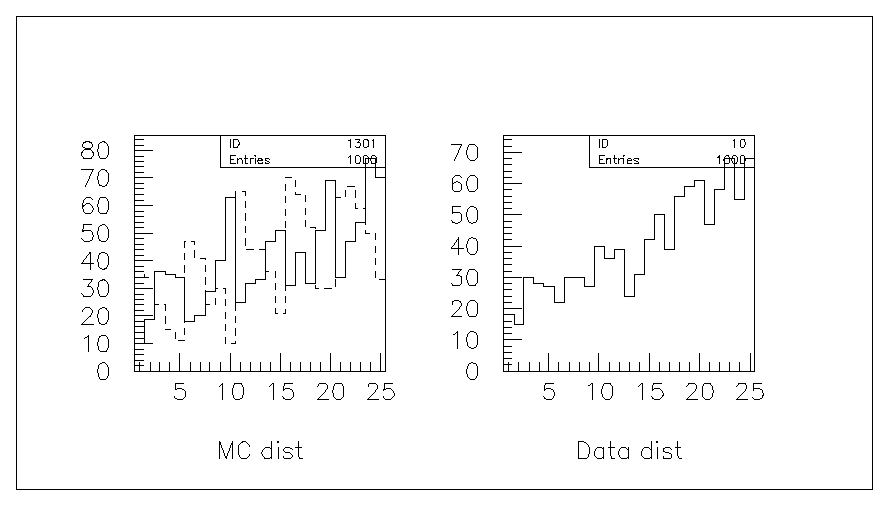
\includegraphics[width=\textwidth]{hmchis.eps}
\caption{Monte Carlo distributions (left) and
         data distribution (right)}
\label{Efield}
\end{figure}
 

\subsection{Example of fits}

\begin{XMP}\baselineskip.95\baselineskip\relax
      SUBROUTINE HEXAM5
*.==========>
*.           OPERATIONS ON HISTOGRAMS AND FITTING
*..=========> (R.Brun, modified by M.Goossens)
      COMMON/HFPAR/PAR(6)
      COMMON/HFGAUS/AG,BG,CG
      DOUBLE PRECISION AG,BG,CG
      DIMENSION X(100),Y(100)
      DIMENSION XF(4000,2),YF(4000),EY(4000),SIGPAR(6)
      DOUBLE PRECISION COV(6,6)
      EXTERNAL HFUNF,HFUNFV,HFUNGA
      CHARACTER*12 TITL1
      DATA TITL1/'TITLE OF ID1'/
*.___________________________________________
*
*             GET hist 110 from data base
*
      CALL HRGET(110,'hexam.dat',' ')
      CALL HRGET(210,'hexam.dat',' ')
*
*
      CALL HBOOK1(1,TITL1,100,0.,1.,0.)
      CALL HCOPY(1,2,'TITLE OF ID = 2')
*
*             Gets information from ID=110 and fills new IDs 1,2
*
      CALL HUNPAK(110,X,'HIST',1)
      CALL UCOPY(X,Y,100)
      CALL VZERO(X(51),50)
      CALL HPAK(1,X)
      CALL HPHIST(1,'HIST',1)
      CALL VZERO(Y,50)
      CALL HPAK(2,Y)
      CALL HPHIST(2,'HIST',1)
*
*             adds 1 and 2. Identifier 3 is created and will contain
*             result of addition
*
      CALL HOPERA(1,'+',2,3,1.,1.)
      CALL HCOPY(3,4,' ')
*
*             Fits 3 with function HFUNF, similar to example 2 .
*             Initializes parameters. Prints results of the last
*             iteration.
*             Superimpose result of fit to the histogram
*             The result of this fit can be compared with the initial
*             parameters of example 2
*
      PAR(1) = 40.
      PAR(2) = 20.
      PAR(3) = 0.4
      PAR(4) = 0.6
      PAR(5) = 0.1
      PAR(6) = 0.1
*
      CALL HFITH(3,HFUNF,'V',6,PAR(1),ST,PMI,PMA,SIGPAR,CHI2)
*
      CALL HPHIST(3,'HIST',1)
*
*
*            Fits a two-dimensional distribution (xf,yf) with HFITN
*            initialize parameters. Prints results of the last
*            iteration.
*            Errors EY automatically computed as SQRT(yf)
*
      NY=0
      DO 10 J=1,40
         DO 5 I=1,100
            CONT=HIJ (210,I,J)
            IF (CONT.EQ.0.) GOTO 5
            NY=NY+1
            YF(NY)=CONT
            EY(NY)=SQRT(CONT)
            CALL HIJXY (210,I,J,X1,X2)
            XF(NY,1)=X1+0.005
            XF(NY,2)=X2+0.0125
    5    CONTINUE
   10 CONTINUE
      PAR(1) = 3.
      PAR(2) = 1.
      PAR(3) = 0.3
      PAR(4) = 0.7
      PAR(5) = 0.07
      PAR(6) = 0.12
*
      CALL HFITV (NY,NY,1,XF,YF,EY,HFUNFV,'V',6,PAR(1),ST,PMI,PMA,
     +            SIGPAR,CHI2)
*       Get covariance matrix of last fit from Minuit.
*       Minuit parameters on 4-byte machines are Double precision 
      CALL MNEMAT(COV,6)
      WRITE(31,*) ' COVARIANCE MATRIX'
      WRITE(31,*) ' *****************'
      DO 20 I=1,6
        WRITE(31,'(6(D12.4,1X))') (COV(I,J),J=1,I)
   20 CONTINUE
*
*       Gaussian fit. Prints first and last iterations.
*
      AG = 2.
      BG = 0.4
      CG = 0.1
      CALL HDELET (0)
      CALL HBFUN1 (1,' ',100,0.,1.,HFUNGA)
      CALL HBOOK1 (5,' ',100,0.,1.,1000.)
      DO 30 I=1,5000
         XR=HRNDM1 (1)
         CALL HFILL (5,XR,0.,1.)
   30 CONTINUE
*
      PAR(1) = 200.
      PAR(2) = 0.4
      PAR(3) = 0.1
      CALL HFITHN(5,'G',' ',3,PAR(1),ST,PMI,PMA,SIGPAR,CHI2)
      CALL HPRINT (5)
      CALL HDELET (0)
*
      END
*
      FUNCTION HFUNF(X)
      COMMON/HFPAR/PAR(6)
      DOUBLE PRECISION A1,A2,C1,C2,XM1,XM2,XS1,XS2,X1,X2
*       Force double precision calculation
      C1  = PAR(1)
      C2  = PAR(2)
      XM1 = PAR(3)
      XM2 = PAR(4)
      XS1 = PAR(5)
      XS2 = PAR(6)
*
      A1=-0.5*((X-XM1)/XS1)**2
      A2=-0.5*((X-XM2)/XS2)**2
      IF(A1.LT.-20.)THEN
         X1=0.
      ELSEIF(A1.GT.20.)THEN
         X1=1.E5
      ELSE
         X1=C1*EXP(A1)
      ENDIF
      IF(A2.LT.-20.)THEN
         X2=0.
      ELSEIF(A2.GT.20.)THEN
         X2=1.E5
      ELSE
         X2=C2*EXP(A2)
      ENDIF
      HFUNF=X1+X2
      END
      FUNCTION HFUNFV (X)
      DIMENSION X(*)
*         Compute function value for 2-dim point X
      HFUNFV = HFUNF(X(1)) + HFUNF(X(2))
      END
      FUNCTION HFUNGA (X)
      COMMON/HFGAUS/AG,BG,CG
      DOUBLE PRECISION AG,BG,CG
      HFUNGA=AG*EXP(-0.5*((X-BG)/CG)**2)
      END
\end{XMP}
\newpage
\begin{Listing}\baselineskip.93\baselineskip\relax
 TITLE OF ID1                                                                    
 HBOOK     ID =         1                                        DATE  18/05/92              NO =    14
      172                                    -
      168                                    I
      164                                    I
      160                                   -I
      156                                   II -
      152                                   II-I
      148                                   I  I-
      144                                 --I   I
      140                                 I     I-
      136                                 I      I
      132                                 I      I
      128                                 I      I-
      124                                -I       I
      120                               -I        I
      116                               I         I
      112                               I         I
      108                               I         I
      104                              -I         I-
      100                              I           I
       96                              I           I -
       92                              I           I-I
       88                             -I             I
       84                             I              I -
       80                             I              I I
       76                             I              I I
       72                             I              I I-
       68                             I              I-II
       64                             I                 I
       60                           - I                 I
       56                           I-I                 I
       52                           I                   I-
       48                          -I                    I-
       44                          I                      I
       40                          I                      I-
       36                          I                       I
       32                          I                       I    -
       28                         -I                       I- - I
       24                       --I                         I-I I
       20                      -I                             I I-
       16                      I                              I-II
       12                     -I                                 I
        8                 - --I                                  I
        4            -----I-I                                    I
 CHANNELS 100   0                                                                                                  1   
           10   0        1         2         3         4         5         6         7         8         9         0   
            1   1234567890123456789012345678901234567890123456789012345678901234567890123456789012345678901234567890   
 CONTENTS 100                          1111111111111                                                                
           10                 112224658012445755432099687543222121                                                  
            1.       211246268181476068282127104785115522257716498                                                  
 LOW-EDGE   1.            111111111122222222223333333333444444444455555555556666666666777777777788888888889999999999
 *10**  1   0   0123456789012345678901234567890123456789012345678901234567890123456789012345678901234567890123456789
 
 * ENTRIES =        100      * ALL CHANNELS = 0.2825E+04      * UNDERFLOW = 0.0000E+00      * OVERFLOW = 0.0000E+00
 * BIN WID = 0.1000E-01      * MEAN VALUE   = 0.3087E+00      * R . M . S = 0.7466E-01

 TITLE OF ID = 2                                                                 
 HBOOK     ID =         2                                        DATE  18/05/92              NO =    15
       84                                                                               -
       82                                                                             - I
       80                                                                             I I
       78                                                                       -     I I  -
       76                                                                       I -   I I  I
       74                                                                       I-I  -I I  I
       72                                                                       I I  II I  I
       70                                                                       I I- II I  I -
       68                                                                       I  I II-I -I-I
       66                                                                    -  I  I-I  I-I  I
       64                                                                  - I  I            I-
       62                                                                  I-I  I             I
       60                                                                  I I -I             I
       58                                                                  I I I              I
       56                                                                  I I I              I
       54                                                                  I I-I              I -
       52                                                                - I                  I I
       50                                                                I-I                  I-I
       48                                                                I                      I
       46                                                                I                      I
       44                                                                I                      I   -
       42                                                               -I                      I-  I
       40                                                              -I                        I  I
       38                                                              I                         I  I
       36                                                              I                         I  I-
       34                                                              I                         I--II
       32                                                              I                             I
       30                                                             -I                             I
       28                                                         -   I                              I  -
       26                                                         I  -I                              I- I
       24                                                         I  I                                I I
       22                                                         I- I                                I I--
       20                                                         II I                                I-I I -
       18                                                         II-I                                    I I
       16                                                         I                                       I-I
       14                                                         I                                         I
       12                                                         I                                         I--
       10                                                         I                                           I
        8                                                         I                                           I - -
        6                                                         I                                           I-I-I
        4                                                         I                                               I-
        2                                                         I                                                I
 CHANNELS 100   0                                                                                                  1   
           10   0        1         2         3         4         5         6         7         8         9         0   
            1   1234567890123456789012345678901234567890123456789012345678901234567890123456789012345678901234567890   
 CONTENTS  10                                                     221233455666557776678686676664543343222221111     
            1.                                                    71850922032539736953183588893942434650812591167574
 
 LOW-EDGE   1.            111111111122222222223333333333444444444455555555556666666666777777777788888888889999999999
 *10**  1   0   0123456789012345678901234567890123456789012345678901234567890123456789012345678901234567890123456789
 
 * ENTRIES =        100      * ALL CHANNELS = 0.2175E+04      * UNDERFLOW = 0.0000E+00      * OVERFLOW = 0.0000E+00
 * BIN WID = 0.1000E-01      * MEAN VALUE   = 0.7102E+00      * R . M . S = 0.1063E+00
\newpage
  MINUIT RELEASE 90.10  INITIALIZED.   DIMENSIONS 100/ 50  EPSMAC=  0.89E-15
 **********
 **    1 **SET EPS  0.1000E-06
 **********
 FLOATING-POINT NUMBERS ASSUMED ACCURATE TO   0.100E-06
     **********************************************
     *                                            *
     * Function minimization by SUBROUTINE HFITH  *
     * Variable-metric method                     *
     * ID =          3  CHOPT = V                 *
     *                                            *
     **********************************************
 Convergence when estimated distance to minimum (EDM) .LT.  0.10E-03
 PARAMETER DEFINITIONS:
    NO.   NAME         VALUE      STEP SIZE      LIMITS
     1 'P1        '    40.000       12.000         no limits
     2 'P2        '    20.000       6.0000         no limits
     3 'P3        '   0.40000      0.12000         no limits
     4 'P4        '   0.60000      0.18000         no limits
     5 'P5        '   0.10000      0.30000E-01     no limits
     6 'P6        '   0.10000      0.30000E-01     no limits
 **********
 **    2 **SET PRINT  0.0000    
 **********
 **********
 **    3 **MIGRAD   1160.       1.000    
 **********
 MIGRAD MINIMIZATION HAS CONVERGED.
 MIGRAD WILL VERIFY CONVERGENCE AND ERROR MATRIX.
 FCN=   81.55959     FROM MIGRAD    STATUS=CONVERGED    391 CALLS      392 TOTAL
                     EDM=  0.21E-05    STRATEGY= 1      ERROR MATRIX ACCURATE 
  EXT PARAMETER                                   STEP         FIRST   
  NO.   NAME        VALUE          ERROR          SIZE      DERIVATIVE 
   1      P1        154.37        3.8591       0.97447      -0.16735E-03
   2      P2        74.934        2.1210       0.51925       0.16237E-03
   3      P3       0.30351       0.15347E-02   0.76783E-03  -0.91430    
   4      P4       0.70017       0.29587E-02   0.17713E-02   0.19339    
   5      P5       0.69299E-01   0.12334E-02   0.28758E-03   0.39057    
   6      P6       0.11985       0.27357E-02   0.62656E-03   0.52392    
 CHISQUARE = 0.9164E+00  NPFIT =   95

 TITLE OF ID1                                                                    
 HBOOK     ID =         3                                        DATE  18/05/92              NO =    16
      172                                    -
      168                                    I
      164                                    I
      160                                   -I
      156                                   I***
      152                                   *I-I
      148                                   I  I*
      144                                 -*I   I
      140                                 I     I*
      136                                 *      I
      132                                 I      I*
      128                                 I      I-
      124                                *I       I
      120                               -I        I*
      116                               I         I
      112                               *         I
      108                               I         I *
      104                              -I         I-
      100                              I           I
       96                              *           I *
       92                              I           I-I
       88                             -I             I
       84                             *              I -                              - -
       80                             I              I*I                        -     I I  -
       76                             I              I I                        I--******  I
       72                            *I              I I-                       I**- II I**I -
       68                             I              I-*I                    - **  I-II-I--**I
       64                             I                 I                  --I* I            *-
       60                           * I                 *                  I * -I             *
       56                           I-I                 I                  I*I-I              I*-
       52                           I                   I-               --*                  I-*
       48                          *I                    *-              I*                     I*
       44                          I                      I             -*                      I-* -
       40                          I                      *-           **                        I **
       36                         *I                       I          *I                         I--I*
       32                          I                       *    -    *-I                             I*
       28                        *-I                       I* - I -**-I                              I-*-
       24                       *-I                         I***I**- I                                I *--
       20                      -I                             I *-II-I                                I-I** -
       16                      *                              I-I                                         I**
       12                    **I                                                                            I**
        8                 - *-I                                                                               I****
        4       ************I                                                                                     I*
 CHANNELS 100   0                                                                                                  1   
           10   0        1         2         3         4         5         6         7         8         9         0   
            1   1234567890123456789012345678901234567890123456789012345678901234567890123456789012345678901234567890   
 CONTENTS 100                          1111111111111                                                                
           10                 112224658012445755432099687543222121221233455666557776678686676664543343222221111     
            1.       21124626818147606828212710478511552225771649871850922032539736953183588893942434650812591167574
 LOW-EDGE   1.            111111111122222222223333333333444444444455555555556666666666777777777788888888889999999999
 *10**  1   0   0123456789012345678901234567890123456789012345678901234567890123456789012345678901234567890123456789
 * ENTRIES =        200      * ALL CHANNELS = 0.5000E+04      * UNDERFLOW = 0.0000E+00      * OVERFLOW = 0.0000E+00
 * BIN WID = 0.1000E-01      * MEAN VALUE   = 0.4834E+00      * R . M . S = 0.2184E+00
 * CHISQUAR  =  0.8156E+02
\newpage
{\scriptsize
     **********************************************
     *                                            *
     * Function minimization by SUBROUTINE HFITV  *
     * Variable-metric method                     *
     * ID =          0  CHOPT = V                 *
     *                                            *
     **********************************************
 Convergence when estimated distance to minimum (EDM) .LT.  0.10E-03

 PARAMETER DEFINITIONS:
    NO.   NAME         VALUE      STEP SIZE      LIMITS
     1 'P1        '    3.0000      0.90000         no limits
     2 'P2        '    1.0000      0.30000         no limits
     3 'P3        '   0.30000      0.90000E-01     no limits
     4 'P4        '   0.70000      0.21000         no limits
     5 'P5        '   0.70000E-01  0.21000E-01     no limits
     6 'P6        '   0.12000      0.36000E-01     no limits
 **********
 **    4 **SET PRINT  0.0000    
 **********
 **********
 **    5 **MIGRAD   1160.       1.000    
 **********
 MACHINE ACCURACY LIMITS FURTHER IMPROVEMENT.

 MIGRAD MINIMIZATION HAS CONVERGED.

 MIGRAD WILL VERIFY CONVERGENCE AND ERROR MATRIX.
 EIGENVALUES OF SECOND-DERIVATIVE MATRIX:
        -0.1596E+01 -0.6458E+00  0.3800E+00  0.7478E+00  0.1277E+01  0.5837E+01
 MINUIT WARNING IN HESSE   
 ============== MATRIX FORCED POS-DEF BY ADDING   1.6018     TO DIAGONAL.
 MIGRAD TERMINATED WITHOUT CONVERGENCE.

 FCN=   1709.709     FROM MIGRAD    STATUS=FAILED       197 CALLS      198 TOTAL
                     EDM=  0.41E+02    STRATEGY= 1      ERR MATRIX NOT POS-DEF

  EXT PARAMETER                APPROXIMATE        STEP         FIRST   
  NO.   NAME        VALUE          ERROR          SIZE      DERIVATIVE 
   1      P1        2.4709       0.73263E-01   0.00000        4.1109    
   2      P2        1.8247       0.37237E-01   0.00000        8.5400    
   3      P3       0.27725       0.24789E-02   0.00000       -125.59    
   4      P4       0.70933       0.51778E-02   0.00000        132.72    
   5      P5       0.90472E-01   0.47875E-02   0.00000       -302.38    
   6      P6       0.21181       0.75383E-02   0.00000       -63.830    

 CHISQUARE = 0.9282E+00  NPFIT = 1848

  COVARIANCE MATRIX
  *****************
  0.5367E-02 
  0.9472E-03   0.1387E-02 
  0.4548E-05  -0.9488E-06   0.6145E-05 
 -0.1520E-04  -0.2581E-04   0.1647E-05   0.2681E-04 
 -0.2597E-03  -0.7556E-04  -0.2361E-06   0.2208E-05   0.2292E-04 
  0.1100E-03  -0.3230E-04  -0.1566E-05   0.1904E-05  -0.2129E-04   0.5683E-04 

     **********************************************
     *                                            *
     * Function minimization by SUBROUTINE HFITH  *
     * Variable-metric method                     *
     * ID =          5  CHOPT =                   *
     *                                            *
     **********************************************
 Convergence when estimated distance to minimum (EDM) .LT.  0.10E-03

 FCN=   69.87250     FROM MIGRAD    STATUS=CONVERGED     64 CALLS       65 TOTAL
                     EDM=  0.38E-05    STRATEGY= 1      ERROR MATRIX ACCURATE 

  EXT PARAMETER                                   STEP         FIRST   
  NO.   NAME        VALUE          ERROR          SIZE      DERIVATIVE 
   1      P1        199.30        3.5192       0.84934      -0.13509E-03
   2      P2       0.39761       0.14150E-02   0.10059E-02   -1.6362    
   3      P3       0.98783E-01   0.10313E-02   0.24990E-03   -1.7442    

 CHISQUARE = 0.1075E+01  NPFIT =   68
}



 EXAMPLE NO = 5                                                                  
 --------------                                                                  
 
                                                                                 
 
 HBOOK     ID =         5                                        DATE  18/05/92              NO =    17
 
      230                                               -
      220                                            -  I
      210                                            I  I
      200                                            ****** -
      190                                          **I  I--*I-
      180                                         *I I    I *I
      170                                        * I-I    I-I*
      160                                       *I-I         I*
      150                                      *I             I*
      140                                      -I              I*
      130                                    -*I               I *--
      120                                    *-I               I--*I
      110                                   *I                     I
      100                                  *I                      *-
       90                                 *I                        *
       80                                *I                         I*
       70                               *I                          I-*
       60                              *-I                           I *--
       50                             *-I                            I-I*I
       40                           -*I                                  **-
       30                         -**                                    I-**
       20                       ***                                        I-***
       10       ****************I                                              I************************************
 
 CHANNELS 100   0                                                                                                  1   
           10   0        1         2         3         4         5         6         7         8         9         0   
            1   1234567890123456789012345678901234567890123456789012345678901234567890123456789012345678901234567890   
 
 CONTENTS 100                               111111111211211121111111                                                
           10                 1 112233456889131356586199288608541122964655231111                                    
            1.    1    2224268062313614000760053587389243868095597245890427768955738341  11        1                
 
 LOW-EDGE   1.            111111111122222222223333333333444444444455555555556666666666777777777788888888889999999999
 *10**  1   0   0123456789012345678901234567890123456789012345678901234567890123456789012345678901234567890123456789
 
 * ENTRIES =       5000      * ALL CHANNELS = 0.5000E+04      * UNDERFLOW = 0.0000E+00      * OVERFLOW = 0.0000E+00
 * BIN WID = 0.1000E-01      * MEAN VALUE   = 0.3984E+00      * R . M . S = 0.9985E-01
 * CHISQUAR  =  0.6987E+02
\end{Listing}
\finalnewpage
\begin{XMPt}{Example of parametrization and smoothing}
\baselineskip.95\baselineskip\relax      SUBROUTINE HEXAM6
*.==========>
*.           PARAMETRIZATION      -     SMOOTHING
*..=========> ( R.Brun )
      DOUBLE PRECISION COEFF
      DIMENSION ITERM(15),COEFF(15)
*.___________________________________________
*
*             Get hist 110 from data base
*
      CALL HRGET(110,'hexam.dat',' ')
*
*       Find best parametrization of histogram in terms of powers
*       of shifted Tchebychev polynomials
*       also produces the corresponding fortran function (here on
*       standard output)
*
*
      CALL HCOPY(110,1,' ')
      CALL HSETPR('PNBX',15.)
      CALL HSETPR('PNCX',15.)
      CALL HSETPR('PLUN',31.)
      CALL HPARAM(1,3011,1.,14,COEFF,ITERM,NCO)
      CALL HPRINT(1)
*
*        ID=2 is smoothed with B-splines
*        statistical errors (sqrt of contents) are drawn
*
      CALL HCOPY(110,2,' ')
      CALL HSPLI1(2,2,14,3,CHI2)
      CALL HIDOPT(2,'ERRO')
      CALL HPHIST(2,'HIST',1)
      END
\end{XMPt}
\finalnewpage
\begin{Listing}
{\scriptsize\baselineskip.95\baselineskip\relax

 ****************************************
 *                                      *
 *   MULTIDIMENSIONAL PARAMETRIZATION   *
 *                                      *
 ****************************************

 FIT CHARACTERISTICS AND OPTIONS
 *******************************

 ID =   1
 DIM =  1
 WORKING SPACE IN /PAWC/ =    5045
  0 USER-DEFINED BASIC FUNCTIONS
  0 USER-DEFINED ELEMENTARY FUNCTIONS
 MAX NUMBER OF REGRESSORS = 15
 MAX POWERS OF POLYNOMIALS IN  EACH DIM = 14  
 AMOUNT OF OUTPUT = 1
 WEIGHTING TYPE = 0
 CLASS OF POLYNOMIALS = 3
 CLASS OF BASIC FUNCTIONS = 0
 BASIC FUNCTION SELECTION MODE = 0
 REGRESSION MODE = 0
 X-NORMALIZATION TYPE = 0
 POWER LIMITOR =  1.00
 F-TEST LEVEL =   1.00
 PARAMETRIZATION SUPERIMPOSED ON HISTOGRAM
 FORTRAN CODE FPARAM WRITTEN ON UNIT 31

 FITTING PROCESS WILL STOP WHEN THE RESIDUAL VARIANCE HITS A MINIMUM

  15 CANDIDATE BASIC FUNCTIONS WERE RETAINED FOR THE FIT
 NUMBER OF POINTS TO FIT =    95
 SUM OF SQUARES OF Y-VALUES =   5000.0    
 MACHINE PRECISION =  0.22E-15


 FITTING PROCESS STOPPED AS RESIDUAL VARIANCE HITS MINIMUM
 R2 =  0.98543      12 REGRESSORS INCLUDED

 FINAL RESULTS OF THE FIT
 ************************

 ITERATION       RSS       R2ADJ     REGRESSOR  COEFF. VALUE   TERM OF PARAMETRIZATION

    13        72.841       0.98350       1        40.320         0 
                                         2       -32.156        20 
                                         3        29.461        60 
                                         4       -20.018        80 
                                         5        7.7912       100 
                                         6       -18.482        50 
                                         7       -7.0469       110 
                                         8       -9.0691        10 
                                         9        4.4675       130 
                                        10        6.4382        90 
                                        11       -3.9874       140 
                                        12        3.1189        30 

\finalnewpage%%%%%%%%%%%%%%%%%%%%%%%%%%%%%%%%%%%%%%%%%%%%%%%%%%%%%%%%%%

 REGRESSOR  STANDARD DEVIATION     CONFIDENCE INTERVAL
     1          0.70650         [  39.144    ,  41.495    ]
     2           1.0509         [ -33.904    , -30.407    ]
     3          0.85147         [  28.044    ,  30.877    ]
     4          0.90853         [ -21.530    , -18.506    ]
     5          0.82336         [  6.4213    ,  9.1611    ]
     6           1.0259         [ -20.189    , -16.775    ]
     7          0.78401         [ -8.3514    , -5.7425    ]
     8           1.0731         [ -10.854    , -7.2836    ]
     9          0.68036         [  3.3355    ,  5.5995    ]
    10          0.83660         [  5.0463    ,  7.8301    ]
    11          0.85716         [ -5.4135    , -2.5612    ]
    12           1.1372         [  1.2267    ,  5.0110    ]
      DOUBLE PRECISION FUNCTION FPARAM (X)
      DOUBLE PRECISION COEFF,P,P0,P1,P2,HELEFT,HBASFT
      DIMENSION X(1),COEFF(12),IBASFT( 1,12)
      DATA COEFF/ 0.40319615E+02,-0.32155589E+02, 0.29460772E+02,
     +-0.20017895E+02, 0.77912196E+01,-0.18481896E+02,
     +-0.70469122E+01,-0.90690550E+01, 0.44674803E+01,
     + 0.64381900E+01,-0.39873663E+01, 0.31188760E+01
     +/
      DATA IBASFT/  0, 20, 60, 80,100, 50,110, 10,130, 90,140, 30
     +/
      FPARAM=0.
      DO 25 K=1,12
      P=1.
      DO 15 I=1, 1
      NUM=IBASFT(I,K)/10
      ITYP=IBASFT(I,K)-NUM*10
      IF (NUM.NE.0) THEN
      IF (ITYP.EQ.0) THEN
      P0=1.
      P1=2*X (I)-1.
      DO 10 J=2,NUM
      P2=2*(2*X (I)-1.)*P1-P0
      P0=P1
   10 P1=P2
      P=P*P1
      END IF
      IF (ITYP.EQ.1) P=P*HELEFT(NUM,X (I))
      IF (ITYP.EQ.2) THEN
      P=HBASFT(NUM,X )
      GOTO 20
      END IF
      END IF
   15 CONTINUE
   20 FPARAM=FPARAM+COEFF(K)*P
   25 CONTINUE
      RETURN
      END
}
\newpage\baselineskip.93\baselineskip\relax
 THIS HISTOGRAM IS FILLED ACCORDING TO THE FUNCTION HTFUN1                       
 HBOOK     ID =         1                                        DATE  17/12/91              NO =  18
      172                                    -
      168                                    I
      164                                    I
      160                                   -I
      156                                   II -
      152                                   I**I
      148                                   *  *-
      144                                 -*I   *
      140                                 I     I-
      136                                 *      *
      132                                 I      I
      128                                *I      I*
      124                                -I       I
      120                               -I        I*
      116                               *         I
      112                               I         I
      108                               I         I *
      104                              -I         I-
      100                              *           I
       96                              I           I *
       92                              I           I-I
       88                             *I             I
       84                             I              I*-                              - -
       80                             I              I I                        -     I I  -
       76                            *I              I I                        I-******** I
       72                             I              I *-                       **I- II I *I -
       68                             I              I-II                    - *I  I-II-I--**I
       64                             I                 I                  --I* I            *-
       60                           * I                 *                  I** -I             *
       56                           I-I                 I                  * I-I              I*-
       52                           I                   I*               -*I                  I-*
       48                          *I                    I-              *                      I*
       44       *                  I                      *             *I                      I-* -
       40                          I                      I-           *I                        I *I
       36        *                *I                       *          *I                         I--*-
       32                          I                       I    -    *-I                             **
       28                        *-I                       I* - I - *-I                              I-*-
       24         *             --I                         I*I I ** I                                I **-
       20                      -*                             ****II-I                                I-I **-
       16          *           *                              I-I                                         I-**
       12                     *I                                                                            I-*
        8           *     -***I                                                                               I****
        4            ******-I                                                                                     I*
 CHANNELS 100   0                                                                                                  1   
           10   0        1         2         3         4         5         6         7         8         9         0   
            1   1234567890123456789012345678901234567890123456789012345678901234567890123456789012345678901234567890   
 CONTENTS 100                          1111111111111                                                                
           10                 112224658012445755432099687543222121221233455666557776678686676664543343222221111     
            1.       21124626818147606828212710478511552225771649871850922032539736953183588893942434650812591167574
 LOW-EDGE   1.            111111111122222222223333333333444444444455555555556666666666777777777788888888889999999999
 *10**  1   0   0123456789012345678901234567890123456789012345678901234567890123456789012345678901234567890123456789
 * ENTRIES =       5000      * ALL CHANNELS = 0.5000E+04      * UNDERFLOW = 0.0000E+00      * OVERFLOW = 0.0000E+00
 * BIN WID = 0.1000E-01      * MEAN VALUE   = 0.4834E+00      * R . M . S = 0.2184E+00
 * CHISQUAR  =  0.7284E+02
 
 THIS HISTOGRAM IS FILLED ACCORDING TO THE FUNCTION HTFUN1                       
 HBOOK     ID =         2                                        DATE  17/12/91              NO =  19
      185                                    I
      180                                    I
      175                                    0
      170                                   II I
      165                                   IIII
      160                                   0IIII
      155                                 III I0I
      150                                 III**I0I
      145                                 00* I*II
      140                                 I*  I *0I
      135                                I*I    III
      130                               III      *I
      125                               I*        *
      120                               0I        I
      115                              I*I        I*
      110                              II          I
      105                              0           0*I
      100                             I*           III
       95                             II           I0* I                                I
       90                             *             II I                        I     I I  I
       85                             I             I *0I                       III  I0 0  I
       80                            *I                II                       0I0I***II I0II
       75                                             I*0                  I I  ****I0I***IIIII
       70                           *                 I I                  III**III0II 0 I**00I
       65                           II                0 *                  00*II I I0I I 0I **0 I
       60                           00                I  *               III*II0    I  I II I *II
       55                          *II                   0I              0I*I 0I               **   I
       50                          0 I                   I*            III*   I                0I*  I
       45                         *I                     I0*           I**I                    I 0* 0I
       40                          I                      I0          I*I                        II**0
       35                        *I                        I* I I I   *I                          00 *  I
       30                       II0                         0** 0 0I**0                           II I**0II
       25                      I*0I                         I0I*****I0I                               0I**0 I
       20                      *II                           I I 0 I0I                                I0 I**0
       15                    I*I                               0 I  I                                      0**0
       10                I0 0*I                                                                              I****0I
        5            ********                                                                                  II0**
 CHANNELS 100   0                                                                                                  1   
           10   0        1         2         3         4         5         6         7         8         9         0   
            1   1234567890123456789012345678901234567890123456789012345678901234567890123456789012345678901234567890   
 CONTENTS 100                          1111111111111                                                                
           10                 112224658012445755432099687543222121221233455666557776678686676664543343222221111     
            1.       21124626818147606828212710478511552225771649871850922032539736953183588893942434650812591167574
 LOW-EDGE   1.            111111111122222222223333333333444444444455555555556666666666777777777788888888889999999999
 *10**  1   0   0123456789012345678901234567890123456789012345678901234567890123456789012345678901234567890123456789
 
 * ENTRIES =       5000      * ALL CHANNELS = 0.5000E+04      * UNDERFLOW = 0.0000E+00      * OVERFLOW = 0.0000E+00
 * BIN WID = 0.1000E-01      * MEAN VALUE   = 0.4834E+00      * R . M . S = 0.2184E+00
 * CHISQUAR  =  0.9674E+02
\end{Listing}
\index{fitting Monte Carlo statistics|)}
\index{Monte Carlo statistics|)}

\endinput

% Local Variables: 
% mode: latex
% TeX-master: "hboomain"
% End: 
